\documentclass[10pt]{book}
\usepackage[utf8]{inputenc}
\usepackage[italian]{babel}
\usepackage{multicol}
\usepackage[bookmarks]{hyperref}
\usepackage[a4paper, total={18cm, 25cm}]{geometry}
\usepackage{listings}
\usepackage{graphicx}
\usepackage{makecell}
\graphicspath{ {./img/} }
\usepackage{color}

\begin{document}
\renewcommand*\contentsname{Indice}
\title{Gestione di Reti}
\author{Federico Matteoni}
\date{A.A. 2019/20}
\maketitle
\tableofcontents
\pagebreak
\section*{Introduzione}
\paragraph{Perché bisogna studiare la gestione?} La situazione corrente comprende: un aumento delle risorse strategiche informative, le reti di computer che da strumento di supporto sono diventate elemento chiave delle organizzazioni, l'aumento esponenziale dei dispositivi interconnessi e aumento anche della complessità e delle funzionalità.\\
C'è quindi richiesta di servizi di rete permanenti e di qualità ottimale, oltre alla necessità di ridurre i costi per le infrastrutture di rete di un'azienda.
\paragraph{Necessità} Gestione di reti eterogenee con l'aiuto dei computer.
\section*{Terminologia e concetti fondamentali}
\paragraph{Managed Objects} Il controllo, la coordinazione e il monitoraggio delle risorse avviene tramite la manipolazione dei cosiddetti \textbf{managed objects}: un MO è una visione astratta di una risorsa che presenta le proprietà dal punto di vista della gestione. Sono \textbf{rappresentazioni astratte di risorse reali}.\\
I confini di un MO specificano quali dettagli sono accessibili ai sistemi di monitoraggio e quali sono schermati (\textbf{black box})

\begin{center}
Management-System $\leftrightarrow$ Managed Object $\leftrightarrow$ Real Object
\end{center}
\begin{list}{}{\textbf{Caratteristiche}}
	\item \textbf{Attributi}: descrivono lo stato/condizione dell'MO, possono cambiare quando cambia lo stato dell'oggetto reale e possono essere manipolati attraverso operazioni di management
	\item \textbf{Operazioni}: consentono l'accesso all'MO. Operazioni tipiche sono get, set, create e delete, ma il numero e tipo delle operazioni influenzano perfomance e complessità dell'oggetto
	\item \textbf{Comportamento}: determina la semantica e l'interazione con la risorsa reale. Normalmente definito in linguaggio naturale
	\item \textbf{Notifiche}: quantità e tipologia dei messaggi, che possono essere generati da situazioni pre-definite da un MO quando avviene una specifica situazione
\end{list}
\paragraph{Management Information Base} L'unione di tutti i MO contenuti in un sistema forma la MIB del sistema. La \textbf{Management Information Base} è la collezione di tutti i management object all'interno del sistema, con i loro attributi.\\
Una MIB deve essere conosciuta sia da chi la implementa che da chi la gestisce.
\subparagraph{Modularità} Gli MO di un sistema sono solitamente definiti in più MIB. Nelle MIB sono introdotti i moduli per consentire un design modulare: moduli diversi possono essere definiti da team diversi, le funzionalità di gestione possono essere estese e modificate\ldots
\paragraph{Paradigma Gestore/Agente}
\begin{list}{}{Agent}
	\item Implementa i MIB delle MO accedendo alle risorse reali
	\item Riceve le richieste da un gestore, le processa e trasmette le risposte appropriate
	\item Smista le notifica riguardanti cambiamenti di stato importanti nel MIB
	\item Protegge gli MO da accessi non autorizzati usando regole di controllo degli accessi e autenticazione della comunicazione
\end{list}
\begin{list}{}{Manager}
	\item Esercita il controllo delle funzioni
	\item Avvia operazioni di gestione tramite opportune operazioni del protocollo per la manipolazione degli MO
	\item Riceve messaggi dagli agenti e li inoltra alle applicazioni interessate per la gestione
\end{list}
\paragraph{Management Protocol} Un protocollo di gestione implementa l'accesso a MO distanti attraverso la codifica di dati di gestione (management data)
\section{lezione 2}
Livello 2 consente di identificare un device sulla rete. In tutte le reti c'è la necessità di identificare la porta di rete. Ogni dispositivo ha almeno un'interfaccia di rete: loopback, che consente di far comunicare processi di rete sulla stessa macchina. \texttt{127.0.0.1} consente di parlare su stessa macchina senza trasmettere sul filo, fondamentalmente un cortocircuito.\\
\texttt{ifconfig} consente di vedere le interfacce di rete disponibili su unix.\\
Se si vuole gestire una rete è fondamentale la standardizzazione.\\\\
Output \texttt{ifconfig}. Parte degli indirizzi, no indirizzo hw su loopback perché il traffico non esce mai (loopback sulla pila OSI è nel livello 3 Network, il MAC address è sul livello 2 Data Link, che non viene toccato da loopback). Indirizzo MAC 6 byte divisi in blocchi dai due punti. I primi 3 identificano il costruttore della scheda di rete. I successivi tre identificano la scheda di rete per il costruttore, che lo setta univocamente. Ciò garantisce univocità. Per primo blocco di tre ho 16M di dispositivi possibili. I MAC address quindi \textbf{non sono univoci}, lo sono \textit{probabilmente}. L'univocità è fondamentale sulla stessa rete. Quindi indirizzo hw identifica univocamente device sulla rete locale. divisi in due blocchi, il primo identifica costruttore della scheda di rete.\\\\
Qualsiasi dispositivo ha indirizzo hw diverso per ciascuna porta.
\section{Ethernet}
Ethernet è un cavo seriale, trasmissione e ricezione. Mezzo seriale. Un filo.\\
Quando si mandano dati non posso tutti insieme ma man mano. Non c'è collisione perché ricezione e trasmissione sono su due fili separati.\\
Pacchetti inviati nel tempo sul filo. Vengono distinti tra loro dal \texttt{preamble}. Pacchetti inviati in una direzione: preambolo, destinazione, sorgente, tipo dei dati, dati effettivi, padding (per rendere pacchetto di 64 se pacchetto è troppo corto), CRC.\\
Quindi per spedire pacchetto necessito di indirizzi (chi voglio e chi sono) e cosa mandare. chi sono lo so, è scritto nella scheda. Voglio conoscere indirizzo di chi voglio.\\
Alla connessione del cavo, se DHCP manda fuori pacchetto per richiesta quindi switch lo impara, se IP statico manda pacchetto ARP quindi switch lo impara.\\
MAC address randomizzato per privacy, spesso e volentieri sui dispositivi mobili.\\
Possibile più di un utente sulla stessa rete con soliti indirizzi, apparati avanzati se ne accorgono.
\section{lezione 3}
un pacchetto è interamente creato dal computer, quindi "non ci si può fidare"\\
Bisogna andare a livello fisico e autenticare, un po' come chiedere la carta d'identità. Metter in atto meccanismi che impediscano di inibire riconoscimento della sorgente.\\
802.1x permette di entrare in rete. Se configurato, il device prima di entrare in rete espone delle credenziali (utente, password, protocollo autenticazione\ldots)\\
Da quel momento in poi \textbf{allegato} al pacchetto c'è il mio nome, ma le informazioni di autenticazione non fanno parte del pacchetto: pacchetti creati quando non c'era preoccupazione e interesse in fattori di sicurezza delle trasmissioni.\\
L'informazione non è parte del pacchetto ma lo riconosce in qualche altro modo il device e \textbf{rimane nel device} (Access Point). Ciò non serve per autenticazione fisica sul cavo: so che sei tu su questo cavo. Ma è necessaria per autenticazione su mezzi condivisi (wifi).\\
Su router MAC cambia ad ogni hop (ethernet comunicazione punto-punto), IP cambia solo se c'è NAT. Le parti da lv 3 in su non cambiano (a meno di frammentazioni\ldots)\\
Robustezza delle reti si fa tramite la ridondanza. Tipico mettere più strade per spedire il traffico: load balancing.\\
Vale sia per corrente elettrica che per traffico di rete.\\\\
\subsection{Aree funzionali}
FCAPS per gestire \textbf{qualsiasi sistema}, da giochi a sistemi di rete. Non sono mutualmente indipendenti.
\begin{list}{}{}
	\item \textbf{Fault Management}: error detection, isolation and repair\\
	Se qualcuno rileva malfunzionamento (riempito disco, ram, sovraccarico CPU\ldots) lo deve notificare
	\item \textbf{Configuration Management}: devo sapere com'è configurato il sistema. Leggere la configurazione è importante, così che le app si possano basare sulle API comuni e funzionare correttamente. Fondamentale capire la configurazione perché permette di definire l'amministrazione, servizi\ldots, possibile riconoscere anche le adiacenze e "questo filo qui va su questa porta qua". che impatto ho se stacco questo cavo, o si rovina? Informazioni sufficenti per amministrare la rete
	\item \textbf{Account Management}: rilevare il consumo di risorse
	\item \textbf{Performance Management}: efficenze e statistiche, performance di sistema sia lato utente sia lato fornitore. Per l'utente è riuscire ad usare la rete, per l'operatore è il giusto compromesso tra investimento sul mezzo e contentezza utente.
	\item \textbf{Security Management}: assicurarsi che ciò che uno fa è effettivamente possibile farlo, autoproteggendosi perché con le reti odierne posso intasare rete (volente o no) e quindi intasare internet, provocando danni
\end{list}
\subsection{Interagire con management object}
Primitive: get, set, create, delete\\
Quando faccio richiesta ad un protocollo mi aspetto una risposta: richiesta -- risposta\\
Contenuto richieste varia durante il transito aggiungendo determinate informazioni. Es: SMS durante il transito aggiunge numero mittente per poter comunicare a destinatario chi inviava.
\subsection{Servizi}
\paragraph{Confermati} Faccio richiesta $\rightarrow$ mi aspetto risposta.\\Es: Telegram/Whatsapp
\paragraph{Non confermati} Faccio richiesta e fine.\\Es: SMS
\begin{center}
	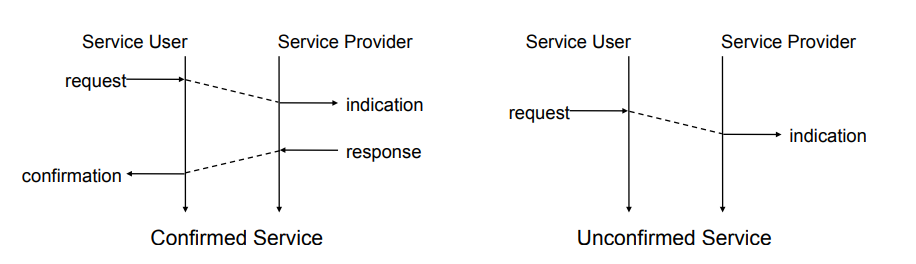
\includegraphics[scale=0.7]{timediag.png}
\end{center}
\subsection{Standardizzazione}
La grande differenza tra ISO/OSI e Internet è il processo di standardizzazione.
\pagebreak
\paragraph{ISO} Nella standardizzazione ISO tutte le varie aziende si accordano su come fare la rete: si creano gruppi di lavoro che si riuniscono (es. ICANN) e producono un documento di lavoro, poi vari comitati lo discutono (fino a qui \textbf{ad alto livello}).\\
Se si mettono d'accordo, pubblicano un \textbf{Draft International Standard} (\textbf{senza implementazione}). Dopodiché, se non viene accettato, creano technical report oppure un \textbf{full standard}.\\
La parte importante è l'assenza di implementazione fino ad avere la creazione dello standard.

\begin{center}
	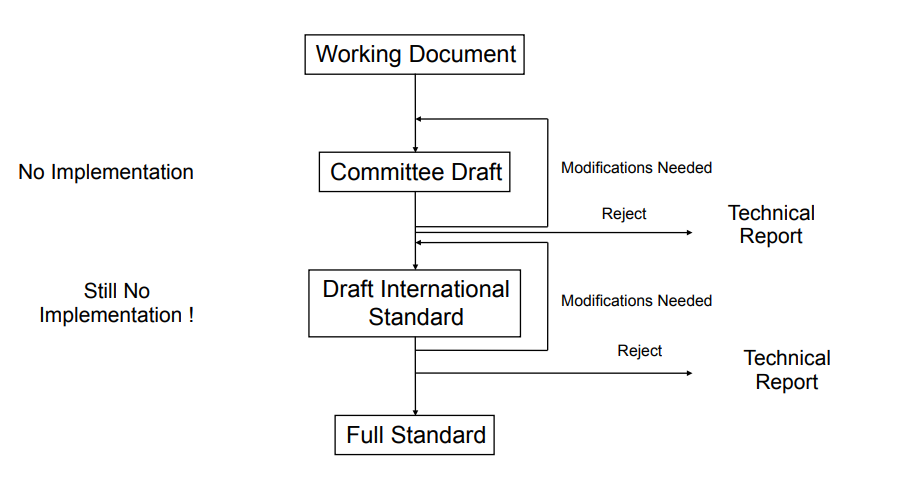
\includegraphics[scale=0.7]{stdiso.png}
\end{center}
\paragraph{Internet} Nella standardizzazione internet è tutto seguito dal comitato IETF, che pubblica aree d'interesse in cui ritiene ci sia possibilità di sviluppo. La sottomissione di un'idea ad un'area d'interesse è libera, oppure si può mandare una mail per idee completamente nuove. Dal working document a draft passa poco e i draft dopo pochi mesi scadono. Dopo massimo due anni o si rifiuta o si fa il draft standard (draft RFC) che o lo si rifiuta o diventa standard in max 4 anni. Necessita di più implementazioni interoperabili.
\begin{center}
	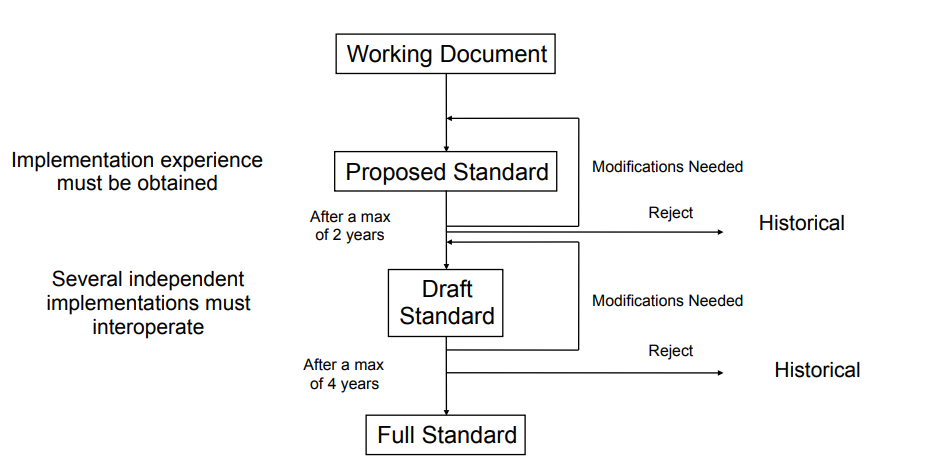
\includegraphics[scale=0.7]{stdietf.png}
\end{center}
\section{Abstract syntax notation one}
\paragraph{ASN1} Sintassi per la definizione di strutture dati e formato di messaggi. Ha l'obiettivo di consentire a macchine dalle differenti architetture hardware di scambiare dati, essere language neutral e consentire la negoziazione della codifica di trasmissione.\\
Come spostare le informazioni? Vari costruttori all'inizio lo facevano "in casa" senza interoperabilità. Col tempo si è reso necessario costruire qualcosa per scambiare le informazioni in maniera interoperabile.
\paragraph{Endian} Come si ordinano i dati in spedizione, per sapere qual è il più significativo.\\
Bit più significativo a sx è big-endian, ormai poco usato. Altrimenti è little-endian.
\section{lezione 4}
Nel monitorare il traffico di rete c'è il problema di come riceverlo. Non sempre siamo nel posto giusto. Se voglio vedere cosa fa altro dispositivo/sottorete a livello di traffico, come faccio? Opzioni: o possiamo mettere la mano sul pc (wireshark) o posso fare finta di essere il pc (chiedendo allo switch, non intrusivamente, di mandare il traffico verso pc pure a me) Prima di iniziare a guardare il traffico, il traffico va visto.\\
\subsection{Common problems with packet capture}
\ldots\\
Perché \texttt{root}? Perché scavalco ciò che fa un'applicazione, perché vedo tutto il traffico indipendentemente dall'applicazione. Per questo devo essere root.\\
Container condivide kernel con host, macchina virtuale emula il kernel.\\
Necessità vedere traffico. Non vorrei mettere mano sulla macchina, perché devo avere so che permette, utente, installare software\ldots\\
Quindi lo faccio da fuori, prelevandolo dallo switch.\\
Metodi software: ho switch, che ha delle porte:
port mirror: tutto traffico diretto verso tale macchina oltre a mandarglielo lo mandi anche a me su questa porta. 1:1 una porta verso una porta, 1:N tot porte switch le mandi qua.
VLAN mirror: simile al port mirror: dammi tutto traffico tale VLAN e mandalo qua
traffic filter/mirroring: dammi solamente traffico di tale porta tale ip\ldots\\\\\\
Singolo cavo ha 2gbps (1gps in upload e 1gbps in dwnld), quindi con port mirror, che posso scaricare al massimo a 1gbps, ho efficacia se traffico sta solo a 1gbps. Dovrei avere scheda di rete da 10gbps per reggere comodamente traffico e non perderlo. Scheda direte più veloce della somma delle due direzioni.\\
Hardware: Network Tap prende le singole direzioni del traffico e ne fa una copia. PC monitor con due schede di rete perché tap divide il filo le direzioni: una prende le direzioni in entrata e una prende la direzione in uscita. Così scopro anche chi invia cosa. Nel port mirror non sono preservate le direzioni.
\section{Lezione}
Software di switch e infrastruttura di rete devono essere duraturi, perché infrastruttura di rete si cambia quando c'è veramente necessità. Altrimenti infrastruttura rimane lì. 
\paragraph{Problema} Gestire le cose nel tempo, che rimangano interoperabili negli anni. Siccome informatica va avanti per mode, si sono posti come problema (fatta negli anni '80) dover gestire qualche sistema non attraverso la url come si fa ora, perché è un modo di fare molto volatile che cambia spesso. Allora hanno fatto standard con negoziazione alto livello: oggetto ha attributi ad alto livello, funzionali al suo funzionamento (macchinettà caffè: c'è acqua, quanti caffè fatti, se ha bicchierini\ldots).\\
Attributi, cosa ti mostro io che sia rilevante per te (non quante viti ha, ma lo stato), operazioni che si possono fare su quegli attributi (accendi, spegni\ldots), comportamento. Software si occupa dell'accensione, non so com'è fatto internamente, io mi limito a chiamare l'operazione. Standardizzazione di funzionamento.
\paragraph{Manager} Comanda l'operazione, impone politica di gestione.
\paragraph{Agent} Gira dentro la macchina gestita e fa cosa chiede manager e solo quello.
\paragraph{Paradigma} Agent gira nella macchina monitorata, e un solo manager raccoglie dati e visualizza.
\paragraph{Come realizzarlo} Bisogna negoziare rappresentazione dati. Per lavorare col web hanno risolto problema scambio dati convertendo tutto a stringhe. Questo modo di fare non ha grandi problemi, ma è inefficiente. Grande quantità di dati per poche informazioni (\texttt{true} scritto invece di un bit). Poco efficiente per tanti dati, chiaro ma non compatto. La URL è breve. Tra due macchine posso scambiarmi dati in maniera binaria, ma bisogna mettersi d'accordo. Se io a 16 bit parlo con una a 64 bit non ci capiamo, quindi bisogna accordarci (Little Endian e Big Endian).
\paragraph{ASN1} Sintassi astratta, implementata dai linguaggi. Quando iniziano a parlare due macchine negoziano rappresentazione e codifica.
\begin{center}
	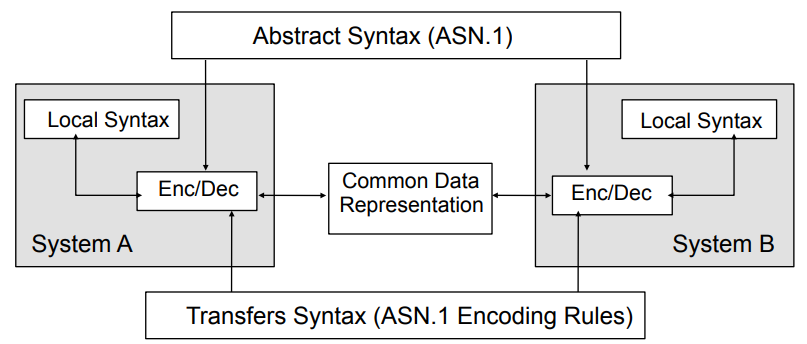
\includegraphics[scale=0.7]{asn1.png}
\end{center}
La sintassi locale (\textbf{local syntax}) è diversa e tipicamente dipendente dal linguaggio utilizzato: ad esempio una in GO l'altra in C, ma anche per sistema A Arduino Nano e sistema B workstation Windows.\\
L'ASN1 quindi definisce una sintassi astratta standardizzata. Permette diverse regole di codifica che trasformano la sintassi astratta in un flusso di byte adatto al trasferimento: \textbf{BER} (Basic Encoding Rules) definisce il mapping tra sintassi astratta e sintassi di trasferimento.\\
ASN1 rimane architettura, idea. La sintassi di trasferimento può essere JSON, GO o qualsiasi altra cosa: l'\textbf{importante è che le due applicazioni si capiscano}.
\begin{list}{}{I \textbf{tipi di dato} (datatypes) primitivi dell'ASN1 sono:}
	\item \texttt{BOOLEAN}
	\item \texttt{INTEGER}
	\item \texttt{BIT STRING}
	\item \texttt{OCTET STRING}
	\item \texttt{OBJECT IDENTIFIER}\\
	Quando trasferisco dati da applicazione ad applicazione, devo poter indicare un campo chiave. Questo tipo di dato identifica univocamente l'oggetto che sto trasferendo all'interno dell'albero ISO
	\item \ldots
\end{list}
\pagebreak
\paragraph{ISO Registration Tree} Usato per identificare univocamente definizioni, documenti, oggetti\ldots Ha una struttura gerarchica, simile ai file system gerarchici. Tutti i nodi di un livello sono univocamente identificati da un numero. Il \textbf{percorso dalla radice al nodo} fornisce una \textbf{sequenza numerica} chiamata \textbf{Object Identifier}.\\
Per esempio, Internet è 1.3.6.1
\begin{center}
	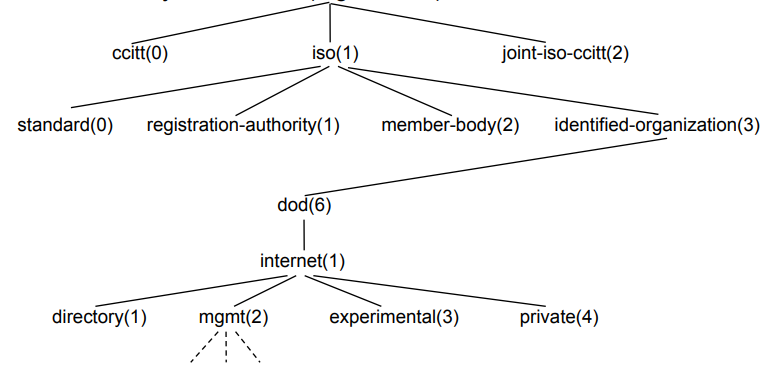
\includegraphics[scale=0.7]{isotree.png}
\end{center}
\textbf{Internet} si trova sotto il \textbf{Dipartimento della Difesa}, che è una \textbf{Organizzazione Identificata} facente parte dell'\textbf{ISO}. Noi parleremo della \textbf{Gestione} (\textbf{m}ana\textbf{g}e\textbf{m}en\textbf{t}) di Internet.\\
L'\textbf{object identifier} quindi, ovvero la sequenza di numeri, risolve il problema dell'identificazione univoca della tipologia dell'oggetto trasmesso sulla rete.
\paragraph{Tipi Complessi} ASN1 ha anche tipi complessi, come \texttt{SEQUENCE OF} che specifica una lista di dati omogenei, o \texttt{REAL} che specifica i numeri reali con mantissa ed esponente dagli \texttt{INTEGER}.
\paragraph{Basic Encoding Rules} Regole di codifica, compattano i dati in una stringa di byte da spedire sul filo. Basato su un algoritmo tag/length/value (TLV), dove ogni variabile è identificata da un tag, la lunghezza del valore in byte e il valore di quei byte. Questo permette al ricevente di ricostruire il tipo del messaggio a partire dal flusso di byte ricevuto.
\chapter{Gestione di Rete}
\section{Nascita}
Gestione di rete nacque, storicamente, nel mondo della telefonia. Necessità di codificare numero, connettersi al centralino, riconoscere il numero\ldots. Standardizzazione necessaria per poter far telefonare a distanze elevate, attraverso le nazioni.\\
La necessità era di un protocollo \textbf{semplice}.
\paragraph{Dati} Poi arrivò internet. Prima bisognava instradare la voce, ora vanno istradati i dati (anche voce, \texttt{VoIP}, ma pur sempre dati). Eredità di tutte le tecnologie e teorie dei tempi della telefonia (es. 5G) ma anche innovazione (es. Browser Web) ma mantenendo il paradigma che era tutto sommato efficiente.
\section{Gestione di Rete Internet}
\paragraph{Cos'è} Sistema di protocolli e tecnologie che permettono di mettere in funzione e controllare un'infrastruttura di rete, per far sì che sia efficiente e che faccia ciò che voglio e che segnali eventuali problemi e comportamenti non previsti.
\paragraph{Reti Geografiche} Questo discorso si applica a reti geografiche, ampie e complesse, che interconnettono un elevatissimo numero di device. Serve anche per far sì che la connessione/disconnessione di dispositivi non crei problemi, e che un utente della rete non possa creare disservizi e potenzialmente tirarla giù.
\paragraph{Anni '90} Il problema principale era mantenere bassi i costi, perché doveva essere pervasivo e poter mettere router in ogni casa. Centraline telefoniche, al contrario, non devono stare in ogni casa.\\
Gli apparati di rete quindi devono costare poco, perciò la gestione di rete non deve costare tanto (nella telefonia costa tanto ed è complicata, quindi "\textit{non facciamo lo stesso errore}": se è semplice anche il costo computazionale è basso, quindi il dispositivo è più economico). Il protocollo, quindi doveva essere \textbf{semplice} e \textbf{efficiente}.\\
Altra cosa importante era \textbf{l'ubiquità} del protocollo: doveva essere disponibile su tutti i dispositivi, così da poterli gestire tutti.\\
Inoltre il protocollo doveva essere \textbf{estensibile}. Almeno \textbf{retrocompatibile}.
\section{SNMP}
\paragraph{Piccoli passi} Il protocollo SNMP è stato progettato di pari passo con il diffondersi di internet, prima a livello universitario e poi industriale. Si è iniziato a sviluppare questo protocollo di gestione dagli albori, perché sin da subito è apparso chiaramente l'importanza che l'infrastruttura stia in piedi.\\
L'SNMP monitora lo stato della rete, per far si che la rete risponda alle esigenze. Ci sono più standard, con primi sviluppati nel 1990.
\paragraph{Semplice} Doveva essere \textbf{semplice}, poiché i sistemi erano semplici, poco potenti e a volte nemmeno multitasking. L'SNMP non poteva girare "in hardware", ma \textbf{necessita di un computer perché necessita di elaborazione dati} e dello stack IP per comunicare. Negli anni '90 lo stack IP non era necessariamente presente sui computer in commercio.\\
La parte importante è che sia \textbf{semplice} e funzionare sotto l'UDP, che è un protocollo estremamente semplice.
\paragraph{Separato} La parte dell'SNMP \textbf{è separata dalla parte di comunicazione} anche se aiuta l'instradamento. \textbf{Non interferisce}, come il cruscotto della macchina (SNMP) col motore (switching).
\paragraph{Trasparente} Sta fuori dalla comunicazione, ma \textbf{deve poterla controllare} e monitorare \textbf{senza interferire}. L'idea è che se l'SNMP viene compromesso lo switch continua a funzionare.
\paragraph{Evoluzione} Nel 1990 viene standardizzata una versione molto semplice: l'\textbf{SNMPv1}. Questa versione fu prodotta in fretta, concentrandosi sulle funzionalità base, in modo da poter entrare subito sul mercato che stava per esplodere.\\
Nle 1991 viene pubblicata la \textbf{Management Information Base}, ovvero l'insieme degli oggetti manipolati tramite l'SNMP.\\
Negli anni successivi ci sono varie evoluzioni del protocollo:
\begin{list}{}{}
	\item \textbf{SNMPv1} supportata da tutti i dispositivi sul mercato
	\item \textbf{SNMPv2} aggiunge poche funzionalità, ma è molto usata soprattutto perché i contatori ora sono a 64bit
	\item \textbf{SNMPv3} aggiunge parecchie funzioni, sacrificando il "\textbf{simple}", quindi non è particolarmente diffuso
\end{list}
\paragraph{Utile} L'SNMP è quindi utile per il monitoring centralizzato su reti estese: è \textbf{importante che questi protocolli siano in funzione in ogni momento}, per riconoscere i problemi in anticipo e avere uno storico della rete per poter fare le verifiche. Anche solo contare il traffico prodotto in termini di byte è un'informazione molto importante.
\paragraph{Agent} \textbf{Apparato di rete}, ad es. nella rete del Fibonacci ci sono diversi agent: access point, computer, stampanti\ldots\\
Sono gli \textbf{oggetti da gestire} e possono cambiare nel tempo: possono essere aggiunti/rimossi, ma possono anche cambiare in tipologia
\subsection{Trap Directed Polling}
Tutti gli agent rispondono ad un manager (solitamente ridondato) $\rightarrow$ $n$ manager per un solo agent.
\begin{center}
	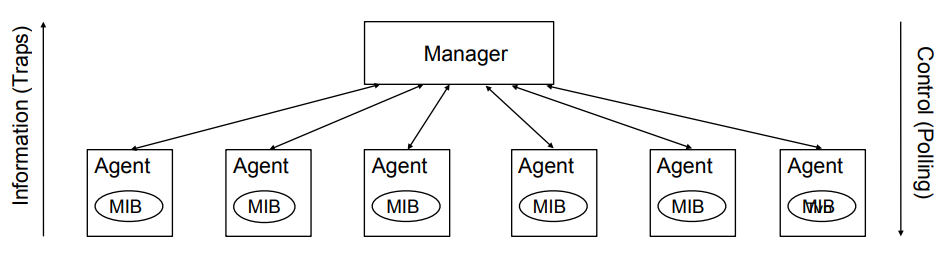
\includegraphics[scale=0.7]{manageragent.png}
\end{center}
\paragraph{Uguaglianza} Con lo stesso protocollo e la stessa funzionalità, devo \textbf{poter controllare dispositivi anche molto diversi}: computer, stampanti, badge, schermi\ldots\\
L'SNMP \textbf{non distingue i dispositivi}, ma \textbf{prende le info dalla MIB} del singolo agent. Ciò che differenzia i vari sistemi operativi, i dispositivi tra loro ecc. sta tutto nella \textbf{MIB} (Management Information Base).
\paragraph{Polling} Controllo. Il manager non comunica continuamente con gli agent, ma esegue un \textbf{polling degli agent}, contattandoli periodicamente per \textbf{ricevere le informazioni aggiornate}.\\
L'SNMP è altamente centralizzato, quindi è compito del manager implementare tutta la funzionalità di monitori e la responsabilità, sicurezza ecc\ldots
\paragraph{Traps} Una volta configurata, sta alla \textbf{periferica avverte il manager se qualcosa non sta funzionando come previsto}. Non informa il manager ogni volta che succede qualcosa (stampo un foglio, prendo un caffè, mi connetto all'Access Point\ldots) perché il manager verrebbe inondato di informazioni, ma \textbf{l'apparato informa il manager se ci sono cose che non funzionano}. Segue la filosofia del "\textit{Se non mandi niente va tutto bene}".\\
Questo può non essere sufficiente, per esempio in caso di problema di rete la comunicazione può non andare a buon fine. In tal caso il polling può risolvere questa cosa, anche se ciò significa apprendere il verificarsi del problema in maniera non tempestiva.
\paragraph{SMI} La struttura delle informazioni di gestione (\textbf{Structure of Management Informativo}, la seconda versione) si basa su un sottoinsieme dei datatype ASN.1 più altri sottotipi:
\begin{list}{}{}
	\item  \texttt{Integer32} interi con il segno
	\item \texttt{Unsigned32} interi senza segno
	\item \texttt{Gauge32} per misure pronte comprese tra min e max
	\item \texttt{Counter32} e \texttt{Counter64} per i contatori: per conoscere la misura effettiva devo fare la differenza tra il valore assunto in due istanti separati.
	\item \texttt{IpAddress} per IPv4
	\item \texttt{TimeTicks} per i centesimi di secondo passati
	\item \texttt{Opaque} che è come il \texttt{void}, non consigliato
\end{list}
Le variabili, inoltre, possono essere
\begin{list}{}{}
	\item \textbf{Scalari}: esistono una sola volta per agent. Es: il nome di un host.
	\item \textbf{Concettuali}: esistono in una tabella concettuale, con valori che cambiano nel tempo.
	\item \textbf{Read} o \textbf{write}, lette o scritte. Non esistono incrementi o reset a valori iniziali, questo per semplicità di protocollo
\end{list}
\paragraph{MIB} Le MIB di SMIv2 sono \textbf{definite tramite speciali macro ASN.1}
\paragraph{Use Case} 
\begin{center}
	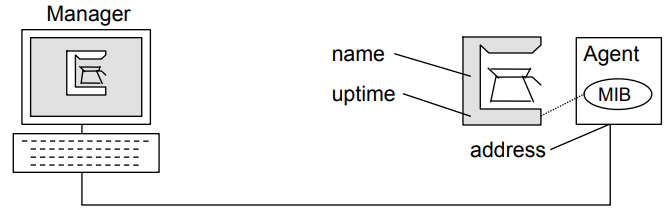
\includegraphics[scale=0.7]{mibusecase.png}
\end{center}
Le variabili sono definite nell'ISO Registration Tree. Una foglia dell'albero rappresente on managed object.
\begin{center}
	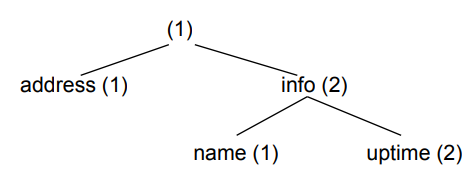
\includegraphics[scale=0.7]{mibusecasetree.png}
\end{center}
\paragraph{Instance Identifier} Ogni managed object è identificato dall'object identifier. Ma tale oggetto ha istanze con determinati valori che cambiano nel tempo: tale istanza è identificata univocamente da un \textbf{Instance Identifier}. La singola istanza di un managed object è \textbf{univocamente identificata concatenando l'Instance Identifier all'Object Identifier}.\\
Gli scalari hanno una sola istanza, e l'istance identifier è \texttt{.0}. Negli altri casi (non identifier) si parte da \texttt{.1}.\\
L'istance identifier è il valore della colonna indice.
\begin{center}
	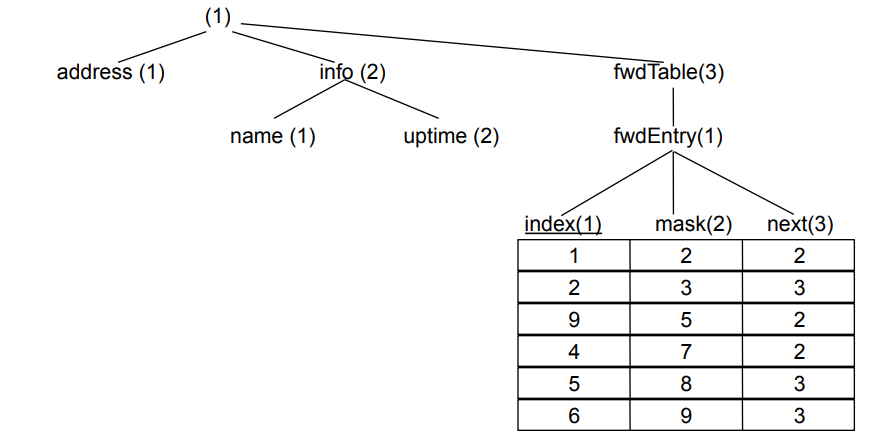
\includegraphics[scale=0.7]{mibusecasetable.png}
\end{center}
In questo caso, per prendere il valore della terza istanza di \texttt{mask}: \texttt{1.3.1.2.9} $\rightarrow$ \texttt{5}.
\begin{multicols}{2}
\begin{list}{}{Altri esempi:}
	\item \texttt{1.3.1.1.1} $\rightarrow$ \texttt{1}
	\item \texttt{1.3.1.2.1} $\rightarrow$ \texttt{2}
	\item \texttt{1.3.1.3.1} $\rightarrow$ \texttt{2}
	\item 
	\item \texttt{1.3.1.1.4} $\rightarrow$ \texttt{4}
	\item \texttt{1.3.1.2.4} $\rightarrow$ \texttt{7}
	\item \texttt{1.3.1.2.7} $\rightarrow$ $\not\exists$
\end{list}
\end{multicols}
\subsection{MIB}
Come si definisce un MIB
\begin{verbatim}
nome DEFINITIONS ::= BEGIN

IMPORT	MODULE-IDENTITY, OBJECT-TYPE, enterprises, IpAddress, TimeTicks	FROM SNMPv2-SMI;
...

END
\end{verbatim}
I nomi servono solo per gli umani, perché sulla rete passano gli object identifier.
\paragraph{Module Identity} Non aggiunge informazione ma indica la versione, questo perché negli anni le reti cambiano ma l'infrastruttura rimane fissa almeno in parte. I device a lungo termine (ad esempio lettori di badge) devono convivere con i nuovi: eterogeneità nelle velocità di elaborazione, protocolli\ldots\\
Non posso togliere oggetto, perché magari versioni precedenti lo usano. Se voglio eliminarlo posso indicarne lo \texttt{STATUS}: obsolete, current o deprecated.
\paragraph{Object Type} \texttt{nome OBJECT-TYPE, SYNTAX, UNITS}\ldots
\paragraph{Notification Type} Invio anche oggetti interessati alle trap\\
linkDown per segnalare se ha perso il link, linkUp per collegamento preso
\begin{center}
	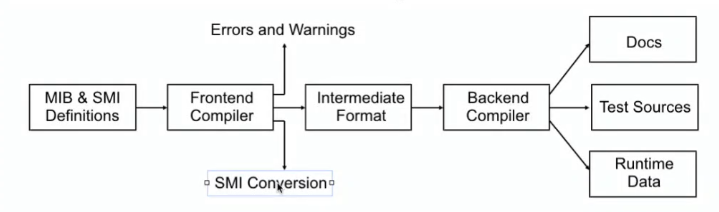
\includegraphics[scale=0.75]{mibcompiler.png}
\end{center}
\paragraph{Utilità dei MIB} Compilatore non è detto che generi linguaggio macchina ma trasforma semplicemente. I \textbf{frontend compilers} SNMP prendono i MIB e producono warning/errori e conversioni di formato SMI
%http://luca.ntop.org/sgr2018/slides/nm2017.pdf
Quando è nato snmp fatti due standard: snmp e mib iniziale (mib-ii, rfc 1213) dove vengono descritti object più importanti per gestione internet.\\
Vogliono controllare stack TCP/IP per vedere cosa non funziona poi monitorare porta di rete. device espongono contatori per interfaccia tramite snmp. contatori byte pacchetti sono base del monitoraggio, ma nel tempo và superato perché contatori su byte sono poco utili: non si sa bene cosa succede però. \\
Obiettivi mib-ii: info base su errori, pochi e semplici control objects (su/giù, errori, pacchett/byte ingresso/uscita), cerca il più possibile di evitare info ridondanti, \textbf{non deve assolutamente interferire con le operazioni} devono essere separati e non rallentare o inficiare in nessuna maniera prestazioni dei dispositivi.\\
Si implementa in hardware, \texttt{eth-tool}. Non si mette a contare i pacchetti, ma è direttamente l'hardware a rispondere. Se chiedo numero pacchetti in un minuto, lui delega all'hardware di contare, quindi il carico non cambia in base al traffico di rete.\\\\
Sono circa 170 oggetti, negli anni alcune def sono troppo semplici, e presuppone IPv4 (IPv6 gestito in mib separati).
\begin{center}
	schema dei MIB-II (1.3.6.1.2)\\
	Albero serve a identificare oggetti.
\end{center}
\paragraph{Composizione} Diviso in gruppi: sistema, interfacce, arptable, componenti stack IP. Anche una parte relativa all'agent SNMP: quante query, errori\ldots\\
La parte trasmissione è aperta, tanti sottoalberi: com'è connesso computer dipende dalla tecnologia, quindi è estensibile a seconda delle nuove tecnologie e cambia nel tempo.\\
Quindi negli anni viene modificato ma è tutto sommato integro sin dalla nascita. Ci sono sovrapposizione fra i MIB\\
Per info più specifiche ci sono MIB successivi. Guardano parte di trasmissione a vari livelli, quindi qualche informazione si può ripetere.
\begin{center}
	tabella
\end{center}
Statistiche su stessa rifa sono a livello diverso, repeater a livello 1. Fanno stessa cosa ma livelli diversi.\\
Per navigare tabelle necessità meccanismo efficiente rispetto a fare tante richieste. Questo perché sistemi modulari, per vedere se valore/elemento esiste.
\paragraph{Ordine lessicografico} \texttt{walk}: lettura consecutiva di oggetti in mib.\\
Leggo oggetti e metto ordinati per numero in ordine lessicografico. Incremento OID e se ho oggetti nel sottoalbero lo visito, da sinistra verso destra. Ricorsivamente, ogni nodo che incontro se ha figli lo visito. Con questo ordinamento si perde la struttura della tabella: \textbf{SNMP lavora solo su questo array ordinato}.
\paragraph{Trap} Unica operazione iniziata dall'agent, che manda direttamente al manager informazioni. Maniera asincrona per informare manager di qualche avvenimento, tipicamente un cambio di stato.\\
\texttt{ifAdminStatus} su \texttt{linkDown} equivale proprio a scollegare fisicamente la scheda di rete. L'\textbf{administrative} è il ciclo di vita, l'\texttt{operational} è operativa. \texttt{ifOperStatus} su \texttt{linkDown} è lo stato e significa che la connessione è caduta.
\paragraph{Estensione dei MIB} Un MIB si può estendere con comandi arbitrari. Ad esempio \texttt{extend test1 /bin/echo "Hello, World!"} eseguirà lo script indicato ogni volta che si esplorerà \texttt{test1} all'interno del MIB \texttt{NET-SNMP-EXTEND-MIB}. Lo script è eseguibile da chiunque abbia accesso alla community a cui è assegnato, quindi bisogna stare attenti alla sicurezza.
\subsection{Primitive}
Due tipi di valori, scalari e tabellari.
\paragraph{Get} Richiesta diretta e precisa di un object identifier\\
Può essere usato per leggere una o più variabili. Basato su UDP, quindi dimensione massima pacchetto: nella risposta bisogna stare attenti alle info. Possibile errore (\textbf{errorStatus)}: tooBig, non entra la risposta nel pacchetto UDP. Altri errori: noSuchName (istanza non esiste o non è foglia, esempio chiedere bicchierini ad una stampante), genErr (qualsiasi altro errore: comunità sbagliata, agent sovraccarico\ldots).\\
\textbf{errorIndex} indica quale delle variabili ha avuto problema. Es \texttt{noSuchName@1} indica che la prima variabile non esiste. Posso fare get con più richieste, quindi errore può essere su altra variabile (es \texttt{noSuchName@3} cioè non esiste il terzo object identifier richiesto ma indica il primo indice fallito, quindi le altre due precedenti esistono ma non vengono ritornati i valori).
\paragraph{GetNext} Richiesta che ritorna l'object identifier successivo a quello chiesto.\\
Non legge istance identifier richiesto ma ritorna il prossimo istance identifier rispetto all'ordine lessicografico. usata per fare discovery delle strutture e leggere le tabelle.\\Nella getNext, nosuchname significa che è finito il MIB (non esiste il successivo). Molto implementation depended, alcuni dopo l'ultimo ritornano il primo invece che noSuchName.
\paragraph{GetBulk} Un po' l'unione di una Get e una GetNext.\\
\texttt{non-repeaters}: di tutti gli OID specificati, indica quanti di essi sono da Get e non da GetNext (i primi \texttt{non-repeaters})\\
\texttt{max-repetitions}: indica il numero di OID dove bisogna fare GetNext (cioè \texttt{max-repetitions} GetNext sui rimanenti)

\paragraph{Set} Scrivere un valore\\
Equivalente in sostanza alla get ma scrivo. Atomica: più valori sono scritti contemporanemante, quindi o vanno bene tutti o non scrivo niente.\\
Errore \textbf{badValue} quando valore scritto è del tipo sbagliato, fuori dal range o comunque non accettabile. Ma anche errore quando oggetto è \texttt{read-only}.\\
noError quando tutto ok, noSuchName quando instance identifier non esiste. Anche qua stesso discorso della get con l'indice.
\paragraph{Trap} Trap dall'agent\\
\textbf{Unico messaggio non richiesto che va dall'agent verso il manager}.\\
Può succedere trap storm, esempio dopo perdita alimentazione tutti dispositivi segnalano riavvio apparati tutti insieme. Se tolgo corrente non posso fisicamente mandare trap, per questo succede quando riavvio e torna su, non quando va giù tutto insieme.\\
Non ci si può fidare totalmente della trap, bisogna fare polling.\\
\texttt{ColdStart}/\texttt{WarmStart} inviate quando avvio un agent (cold da freddo, spento, caso tipico, invece warm è da riavvio)\\
\texttt{LinkDown}/\texttt{LinkUp}\\
\texttt{AuthenticationFailure} quando faccio richiesta posso non avere autorizzazioni, trap segnala al manager della situazione (tipicamente se provo tante password una dietro l'altra).\\
\texttt{EnterpriseSpecific}, vedi valore enterprise e specific nel formato del pacchetto. ad esempio fine carta di una stampante. Specific=1 per dire che l'interpretazione è a seconda del mib.
\begin{center}
	Formato pacchetti
\end{center}
Community: una sorta di password, vedo se utente che richiede è abilitato a certa operazione. PDU payload data unity\\
Get getnext e set ricevono getresponse tutte e tre.\\
Importante sapere IP host che manda trap (potrebbe vederlo dal pacchetto UDP), perché l'ip nell'udp può essere mascherato o cambiato ad esempio dal nat\\\\
\texttt{sysDescr}(1) breve descrizione del sistema (stringa, \textbf{arbitraria})\\\\
\texttt{sysObjectID}(2) identifica sia modello che costruttore, per riconoscerlo e andare nel relativo MIB o, ad esempio, mettere l'icona giusta.\\\\
\texttt{sysUptIme}(3) da quanto è attivo l'\textbf{agent} (non è per forza identico a quello di sistema). Serve anche per poter leggere correttamente le variabili \texttt{gauge} per esempio, per fare la differenza per sapere quanto è cambiato il valore nell'ultimo minuto (ad esempio). Ma non posso aspettarmi che il nuovo valore sia maggiore (es: è saltata la corrente, oppure se il contatore ha fatto wrap (fine dei bit e ripartito da 0)) Quindi devo distinguere riavvio agent da wrap, non posso fare semplice differenza perché potrei tirare fuori numero sbagliato (es negativo, ma valore \texttt{unsigned} fa diventare grandissimo). Per sapere se si è riavviato agent o se contatore ha fatto wrap uso \texttt{sysUpTime}.\\\\
\texttt{sysContact}(4) chi contattare.\\\\
\texttt{sysName}(5)\\\
\texttt{sysLocation}(6)\\\\
\texttt{sysServices}(7) dà info sui servizi gestiti dal sistema. Stringa di bit che identifica a quale livello ISO/OSI si trova il sistema
\paragraph{Gruppo \texttt{interfaces}}\begin{list}{}{Informazioni sulle interfacce di rete}
	\item \texttt{ifIndex} da indice interfaccia di rete. Non sono consecutivi, se aggiungo o rimuovo porte numerazione non cambia.
	\item \texttt{ifDescr} che descrive cosa fa l'interfaccia 
	\item \texttt{ifType} il tipo di interfaccia, eth, wireless...
	\item \texttt{ifMTU} la Maximu Transmission Unit. La frammentazione (livello IP) la fa chi riceve un pacchetto deve spedirlo su una linea con MTU più piccolo
	\item \texttt{ifSpeed} la velocità attuale dell'interfaccia
	\item \texttt{ifPhysiAddress} indirizzo fisico, il MAC
	\item \texttt{ifAdminStatus} indica se l'interfaccia è fisicamente presente o meno
	\item \texttt{ifOperStatus} indica se l'interfaccia è operativa (accesa, up\ldots)
	\item \texttt{ifLastChange} valore del \texttt{SysUptime} dell'ultima volta che l'interfaccia di rete ha cambiato stato
	\item \texttt{ifInOctets} numero ottetti in ingresso alla porta
	\item \texttt{ifInUcastPkts} pacchetti unicast
	\item \texttt{ifInNUcastPkts} pacchetti non unicast
	\item \texttt{ifInDiscards} pacchetti scartati
	\item \texttt{ifInErrors} pacchetti in errore
	\item \texttt{ifInUnknownProtos}
	\item \texttt{ifOutOctets} numero ottetti in uscita alla porta
	\item \texttt{ifOutUcastPkts} pacchetti unicast
	\item \texttt{ifOutNUcastPkts} pacchetti non unicast
	\item \texttt{ifOutDiscards} pacchetti scartati
	\item \texttt{ifOutErrors} pacchetti in errore
	\item \texttt{ifOutQlen} numero di pacchetti in coda in uscita. Dovrebbe essere 0 o quasi, altrimenti interfaccia non riesce a spedire i dati al giusto ritmo
	\item \texttt{ifSpecific}
\end{list}


\paragraph{enp0s1} Perché si chiama così? Dà informazione su dove si trova la scheda
\paragraph{Gruppo \texttt{arp}} Informazioni sulla risoluzione dei nomi. Riempita automaticamente dallo switch: su quali interfacce ha scoperto quali indirizzi fisici. Non è una corrispondenza delle porte, è dell'ARP.
\subsection{SNMPv2}
Usato snmpv2 invece che v1 perché aveva problemi strutturali: il primo sono i contatori a 32bit che sono molto limitati per la tecnologia odierna (10-100Gbit il contatore si "riempie" molto velocemente). Inoltre nella v2 c'è tutto quello scartato in v1 per questioni di tempo (necesario fare protocollo in fretta)
\paragraph{Primitive di SNMPv2} Sono tutto sommato le stesse con \texttt{GetBulk} e \texttt{Inform}
\begin{list}{}{}
	\item \texttt{GetBulk} per richieste più efficienti per massimizzare numero richieste in un pacchetto. Metà strada tra \texttt{Get} e \texttt{GetNext}. Oltre OID due parametri:
	\begin{list}{}{}
		\item \texttt{non-repeaters}: di tutti gli OID specificati, \texttt{non-repeaters} indicano quanti di quelli sono quelle variabili a cui applicare una \texttt{Get} secca e non in sequenza. Dei restanti, devo fare \texttt{max-repetitions} \texttt{GetNext}
		\item \texttt{max-repetitions} quante \texttt{GetNext} applicare
	\end{list}
	Se chiedo poche cose non risparmio molto rispetto ad una \texttt{GetNext}, se chiedo troppe cose (\texttt{max-repetitions} troppo alto) devo stare attento che entri tutto in un pacchetto.
	\item \texttt{Inform} è una sorta di \texttt{Trap} informata perché riceve una \texttt{response}. Altra differenza è che la \texttt{Inform} la può mandare sia un Manager (che può informare un Manager di livello superiore, per esempio) che un Agent
\end{list}
\paragraph{Formato} Hanno la stessa PDU ma con modifiche all'interno, però sostanzialmente è uguale
\paragraph{Eccezioni} A differenza degli errori di SNMPv1 sono più esplicativi. Ad esempio \texttt{noSuchName} spacchettata in \texttt{noSuchObject}, \texttt{noSuchInstance} o \texttt{endOfMibView}. Sono un \textbf{raffinamento dei codici di errore di SNMPv1} e un \textbf{miglioramento delle primitive}.
\paragraph{Differenze principali} Più velocità con la Bulk, contatori a 64bit, errori molto più dettagliati. Ma \textbf{non risolve granché} in termini di sicurezza.
\subsection{SNMPv3}
\paragraph{Obiettivi} Bisogna risolvere problemi di sicurezza soprattutto per la \texttt{Set}. Inoltre bisogna fare il design di un'architettura a lungo termine.\\
Supportare implementazioni sia complesse che semplici (\textbf{scalabilità}).\\
Il tutto \textbf{rimanendo il più semplici possibile}. Nella realtà non è stato così, e la diffusione è ancora molto limitata con la maggior parte delle reti che continuano ad usare v1 e v2.
\paragraph{Architettura} Tanti componenti, rimovibili e intercambiabili. Vuoti se una certa implementazione non la supporta, rimovibili a seconda di cambiamenti tecnologici o di implementazione.
\begin{center}
	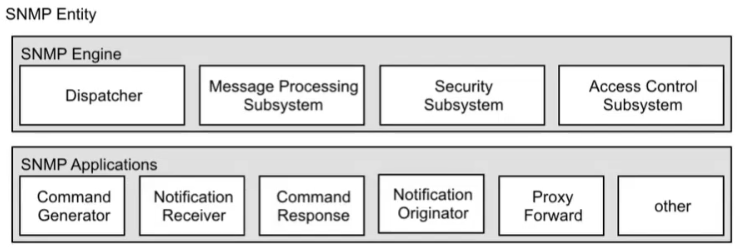
\includegraphics[scale=0.75]{snmp3.png}
\end{center}
Supporta vari tipi di protocollo per lo scambio di messaggi e per il sistema di sicurezza (comunità, utente, "\textit{altro}")
\paragraph{Caratteristiche più importanti} 
\begin{enumerate}
	\item \textbf{Sicurezza}\\
	Il messaggio è autentico? Data Integrity e Authentication\\
	Tramite una funzione hash, con chiave simmetrica faccio l'hash dei dati e calcolo un MAC (Message Autethication Code) es MD5. Pacchetto diventa User (key), MAC e Data.\\
	Il ricevente ricalcola l'hash e se MAC calcolato e ricevuto sono uguali allora apposto.\\
	Il problema è la \textbf{chiave simmetrica}.
	\item \textbf{Protezione dalla ripetizione di vecchi messaggi}\\
	Il ricevente conosce l'orario del messaggio ricevuto, se il messaggio ricevuto è nell'intervallo di validità e \textit{più giovane} dell'ultimo messaggio valido, allora è processato e l'orologio viene aggiornato. Quindi, ad inizio comunicazione gli orologi vengono sincronizzati.
	\item \textbf{Protezione dallo sniffing}: si crittano i dati
\end{enumerate}
\begin{center}
	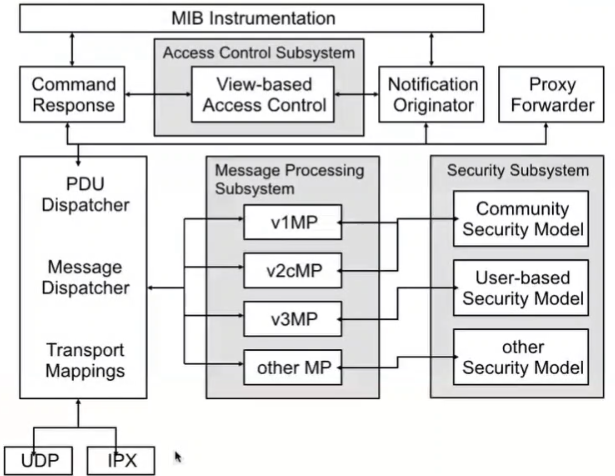
\includegraphics[scale=0.75]{snmp3arch.png}
\end{center}
\paragraph{Messaggi} Possedendo, tra le altre cose, il supporto all'encryption, SNMPv3 ha un formato dei messaggi completamente diverso dalle versioni precedenti. Può essere un problema, in particolare per chi scrive i device: la complessità per implementarlo è sicuramente diversa.
\begin{center}
	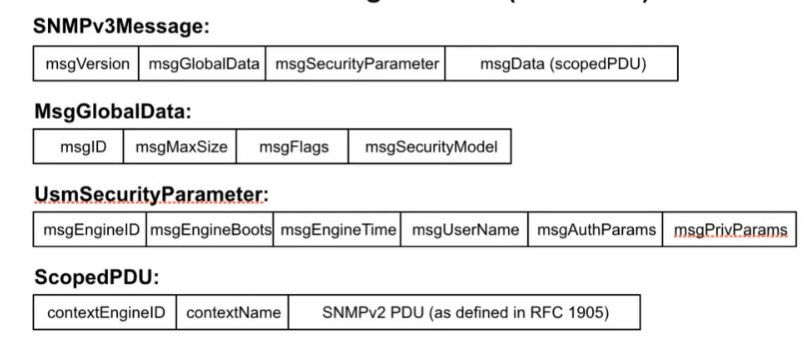
\includegraphics[scale=0.75]{snmp3msg.png}
\end{center}
\paragraph{Proxy Agents} Permettono ai manager di accedere ad altri agent non accessibili direttamente (es dietro firewall) o accessibili mediante protocolli non IP (es IPX)
\begin{center}
	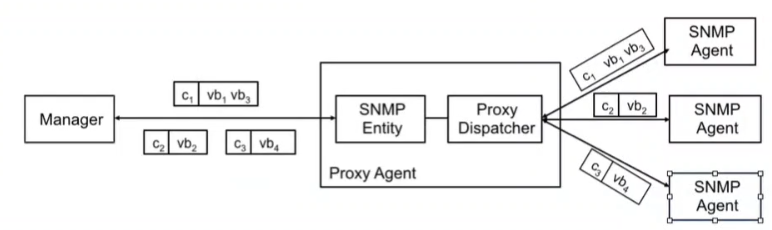
\includegraphics[scale=0.75]{snmp3proxyagents.png}
\end{center}
Le applicazioni di management devono, solitamente, selezionare le opportune stringhe di comunità o contesto, così da abilitare il proxy a raggiungere gli agenti (non c'è trasparenza). I proxy sono importanti per l'implementazione dei firewall o per conversioni tra diverse versioni di SNMP.
\paragraph{Agent estensibili} Il master agent è un agent vuoto, senza variabili all'interno. Il subagent è l'agent stesso, che implementa il MIB.
\begin{center}
	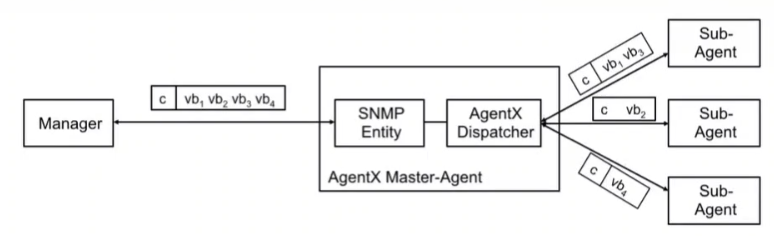
\includegraphics[scale=0.75]{snmp3agentestensibili.png}\\
	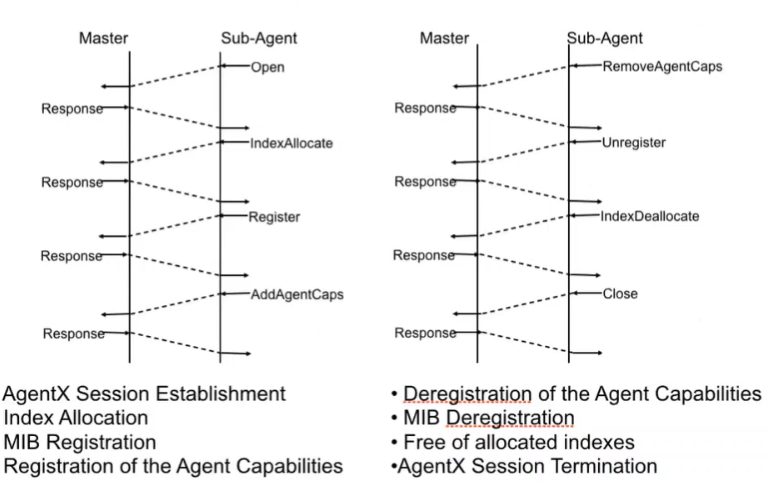
\includegraphics[scale=0.6]{snmp3agentestensibili2.png}
\end{center}
SubAgent fa la open, a cui il Master risponde con la response.\\SubAgent poi comunica, con la IndexAllocate, quali OID implementa. Il Master vedrà se nessun altro ha richiesto gli stessi OID, in caso risponde al SubAgent, che risponderà registrandosi e in caso con altre capabilities.\\
Quindi \textbf{ogni subagent specifica al master cosa implementa}.\\
ASN1 finisce a SNMP entity, nella parte successiva c'è il protocollo AgentX, molto più semplice su TCP.
\chapter{Rete Cellulare}
Quando telefono si connette a rete mobile il gateway lo autentica.\\
GTPC realizza autenticazione, il telefono si annuncia sulla rete (register) e disannuncia quando esce, oppure update quando cambia cella. L'annuncia comprende il MEI (identificativo univoco del telefono), IMSI (international mobile subscriber identity) e altre info, ad  esempio sul profilo tariffario (velocità max ad es). Sulla rete passano anche info su nodo di rete e identificativo della cella. Le informazioni sono ricavate e comunicate dal provider e dal GTPC, non dal telefono. Ad esempio, il numero di cellulare è dato dal protocollo, non è memorizzato sulla SIM.\\
Create session crea la connessione e la stabilisce.\\
Protocollo GTP inoltre negozia i \textbf{tunnel}: permettono che cambiando cella cambiano i parametri della connessione ma la comunicazione rimane. Pacchetti incapsulati in tunnel GTP, io continuo a vedere il mio ip verso l'esterno e percepisco come se fosse rete fissa.\\\\
Traffico è incapsulato dentro il pacchetto GTP.
\paragraph{Analisi traffico radio} Per analizzare il traffico radio delle reti mobili (ad esempio, tramite Wireshark) su smartphone si può implementare una "VPN senza VPN": cioè i pacchetti vengono catturati dal sistema operativo per mandarli su una VPN che in realtà è la rete mobile stessa.
\chapter{RRDtool}
\section{RRDtool Database}
I db relaz hanno tabelle connesse con relazioni\ldots con inserimento, cancellazione e aggiornamento. Questo non è abbastanza. Inoltre su uso questo modo la tabella cresce all'infinito, durante il monitoraggio\\
Poi DB relaz non efficienti nel fare aggregazione nel tempo dei valori. Inoltre, i dati più vecchi diventano via via meno importanti.
\paragraph{RRDtool} Padre di tanti DB a sede temporale. RR=Round Robin. RRD è un \textbf{file}, in un formato particolare:
\begin{list}{}{}
	\item \textbf{Static Header} che indica cosa contiene, ultimo timestamp di aggiunta e ultimo dato aggiunto\ldots
	\item \textbf{Live Header} 
	\item \textbf{Round Robin Archive} specifica che tipo di dato mantenere per quanto tempo e con che risoluzione misurare
	\item \textbf{Round Robin Archive}\ldots
	\item \ldots altri RRA
\end{list}
\paragraph{RRD} Array circolare con numero fisso di slot di storage.
\begin{center}
	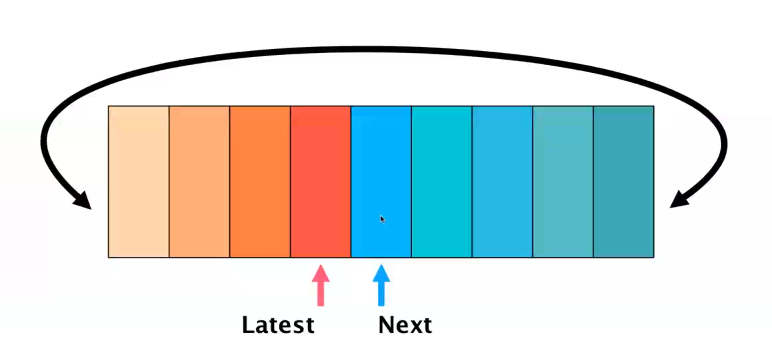
\includegraphics[scale=0.7]{rrdtool_rr.png}
\end{center}
\paragraph{Data Source} Qualsiasi cosa con numeri, file di log, contatori SNMP\ldots
\paragraph{Sconosciuto} Come gestire \texttt{UNKNOWN}? Unknown non è 0, è contagioso (1+unknown = unknown). RRDtool gestisce gli unknown, configurabile quanto unknown ignorare (default: 50\%) e come gestirli
\paragraph{Archivi multipli} Tieni i dati pronti alle giuste risoluzioni\\
Media su 5 minuti per un giorno.
Massimo su 1h per un mese
\paragraph{Anomaly Detection} Per accorgersi di problemi, soglie: colorare grafici in base a soglie (sopra 60 giallo, sopra 85 rosso ad esempio). Però sono statici.\\
Altrimenti in base ai valori storici: vedo qual'è la media nel passato e se mi discosto tanto\ldots\\
Una cosa interessante che fa RRDtool. La \textbf{derivata} da indicazione di quanto mi discosto dall'osservazione precedente: 0 è costante, numeri più alti indicano grandi variazioni dall'osservazione precedente. Quindi la prima domanda è quanto tempo osservare. Anche dalla natura della metrica: una derivata violenta può significare problemi al sensore, in altre metriche può essere normale (trasmissione, attività processore\ldots).\\
Inoltre la derivata su altre misure possono anche essere molto ampie senza che sia allarmante: download/upload, ad esempio. Dipende molto da cosa misuro: derivata su più intervalli o solo sulla precedente misura?\\
Però il color-coding: verde ok, giallo mh e rosso male male, è ottimo. Keep it simple, seplicativa e semplice è meglio di troppi valori disaggregati.\\\\
Nella pratica, l'\textbf{anomaly detection} consiste nel fare una istantanea del sistema monitorato in due momenti diversi e vedere quanto differiscono i due momenti, interpretando le differenze.
\paragraph{Holt-Winters} Media mobile stagionale. \begin{list}{}{Parametri:}
	\item $\alpha$
	\item $\beta$
	\item Periodo di analisi
\end{list}
All'interno dell'array di valori si crea le bande.
\begin{list}{}{tutti valori letti dalla scheda di rete}
	\item ifindex: identifica l'interfaccia
	\item ifdescr: descrizione interfaccia (ad es: eth0 ma anche descrizioni significative)
	\item iftype: tipo interfaccia (ethernet, \ldots)
	\item ifmtu: maximum transfer unit, indicata per poter evitare cattive configurazioni nell'mtu. MTU deve essere la stessa perché se uno trasmette a $>$ mtu di uno dei due non comunicano più
	\item ifspeed: 
	\item ifphysaddress: indirizzo fisico della porta di rete, mac address della porta dello switch
	\item ifadminstatus: se scheda è fisicamente presente sullo switch
	\item ifoperstatus: per una scheda presente, se è operativa oppure no
	\item iflastchanged: sysuptime dell'ultima volta che l'interfaccia è cambiata di stato
	\item ifinoctets: otteti in
	\item ifinucastpkts: unicast in
	\item ifinnucastpkts: not-unicast in
	\item ifindiscards: discarded in
	\item ifinerrors: errori in
	\item ifinunknownprotos: sconosciuti in
	\item ifoutoctets: otteti out
	\item ifoutucastpkts: unicast out
	\item ifoutnucastpkts: not-unicast out
	\item ifoutdiscards: discarded out, dipende dall'implementazione della scheda
	\item ifouterrors: errori out, dipende dall'implementazione della scheda
	\item ifoutqlen: stessa info del comando \texttt{netstat} e simili, info sulle code in uscita
	\item ifspecific:
\end{list}
router frammenta il pacchetto quando mtu della linea ricevente è più piccolo. ma può essere che mittente mandi pacchetti frammentati quando qualcuno chiede a lui di mandare pacchetto troppo lungo rispetto mtu.\\
Frammentazione è concetto dell'IPv4\\
TCP frammentazione non c'è ma non perché non si possa fare, ma perché un pacchetto TCP non può essere frammentato (è indicazione di errore che qualcosa nel TCP non ha funzionato). Path MTU discovery (PMTUD), pacchetti sempre più grandi finché non si trova dimensione massima con l'\textbf{obiettivo di evitare la frammentazione}. Perché meccanismi TCP permettono di farlo. UDP pacchetti vivono di vita propria quindi può succedere frammentazione.\\
Pacchetti non unicast sono "problematici" perché riempino le porte dello switch.
\chapter{Bridge MIB}
Bridge è mettere assieme due interfacce di rete\\
Risponde alla domanda: come fare per iniziare a vedere la topologia della rete e, quindi, i dispositivi collegati ad un host?\\
Attraverso bridge-mib per la topologia di rete. Importante anche per inquadrare che impatto può avere un'allarme sul sistema. Così so sia quali sono i nodi principali ma anche l'impatto di qualche problema: se cade una macchina che collega tante altre macchine, cadono tutte, mentre se cade no nodo marginale il problema è più contenuto.
\chapter{Cattura}
\begin{center}
	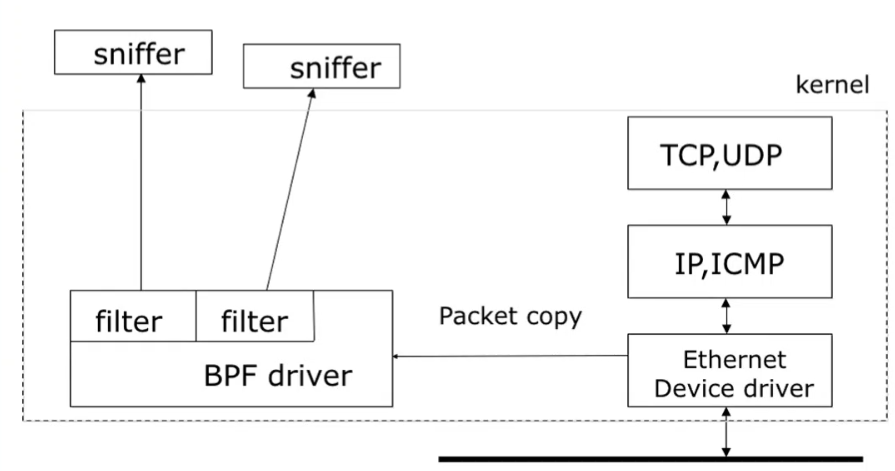
\includegraphics[scale=0.75]{cattura.png}
\end{center}
Quando cattura traffico intervengo sul traffico e me lo copio verso l'applicazione che cattura ciò che sarebbe destinato ad altri. Quindi ethernet copia pacchetto al BPF driver che, tramite filtri, manda copie agli sniffer.\\
Gli sniffer necessiterebbero di diritti su
\paragraph{Capabilities} Quando uno è SU ha diritti eccessivi rispetto a ciò che deve fare, quindi le \textbf{capabilities} sono le possibilità di spezzare i diritti di amministrazione in categorie: non c'è bisogno di essere root che fa veramente veramente tutto perché se ne può abusare. Quindi il concetto di root è spacchettato in varie possibilità: configurazione del MAC address, Net Admin\ldots\\
Un'app quindi dovrebbe nascere con conetto di capabilities e avere diritti minimi necessari per fare ciò che vuole/deve fare.
\paragraph{Filtro} Devo indicare l'interfaccia a cui sono interessato catturare pacchetti (eventualmente tutte) e in caso che tipo di pacchetti ricevere. Così il BPF driver \textbf{non} invia all'applicazioni pacchetti non interessanti, perché anche scartare qualcosa richiede tempo.\\
BPF e sottosistema è localizzato nel kernel. Solamente la parte del pacchetto è inoltrata, il resto (filtro e copia dei pacchetti) è nel kernel.\\
Nel mondo linux, la cattura dei pacchetti equivale ad aprire un socket.
\section{\texttt{libpcap}}
\paragraph{\texttt{pcap\_open\_live}} Parametri: \texttt{deviceName} scheda di rete, \texttt{maxCaptureLen} lunghezza massima del pacchetto (sia per efficienza, sia per privacy se non ho bisogno dell'intero pacchetto), \texttt{setPromiscuosMode} per abilitare la modalità promiscua (cattura tutto il traffico sulla scheda), \texttt{pktDelay} non c'erano i thread quindi hanno pensato di mettere un tempo massimo per cui aspettare un pacchetto e in caso ritornare senza valore, \texttt{errorBuffer} sempre per ragioni storiche se la \texttt{pcap\_open\_live} fallisce il buffer contiene la ragione per cui è fallita\\
\texttt{live}: leggo traffico di rete in tempo reale. C'è la possibilità di aprire file \texttt{pcap} per leggere traffico salvato su file.\\
%TODO problema del pcap
In realtime bisogna controllare il tempo del pacchetto con il mio tempo. L'orario contenuto nel pacchetto è quello della sua ricezione, quindi nell'rrd è registrare i dati all'orario del pacchetto, non a quello di sistema
\paragraph{\texttt{pcap\_compile}} Compila l'espressione del filtro
\paragraph{\texttt{pcap\_setfilter}} Trasferisce nel kernel l'espressione compilata
\paragraph{\texttt{pcap\_next}} Prende il prossimo pacchetto catturato
\paragraph{Offset} Offset del pacchetto all'interno di Wireshark sarebbe il byte (esempio offset 12 $\rightarrow$ byte 12)
\paragraph{BPF} Un esempio di filtro BPF compilato (TCP, in questo caso) \begin{lstlisting}
(000) ldh      [12]
(001) jeq      #0x86dd          jt 2 jf 7
(002) ldb      [20]
(003) jeq      #0x6             jt 10 jf 4
(004) jeq      #0x2c            jt 5 jf 11
(005) ldb      [54]
(006) jeq      #0x6             jt 10 jf 11
(007) jeq      #0x800           jt 8 jf 11
(008) ldb      [23]
(009) jeq      #0x6             jt 10 jf 11
(010) ret      #262144
(011) ret      #0
\end{lstlisting}
Di seguito un esempio UDP \begin{lstlisting}
(000) ldh      [12]
(001) jeq      #0x86dd          jt 2 jf 7
(002) ldb      [20]
(003) jeq      #0x11            jt 10 jf 4
(004) jeq      #0x2c            jt 5 jf 11
(005) ldb      [54]
(006) jeq      #0x11            jt 10 jf 11
(007) jeq      #0x800           jt 8 jf 11
(008) ldb      [23]
(009) jeq      #0x11            jt 10 jf 11
(010) ret      #262144
(011) ret      #0
\end{lstlisting}
\begin{list}{}{}
	\item \texttt{jeq} Jump if equal
	\item \texttt{jt}, \texttt{jf} Jump if true, jump if false
	\item \texttt{ldh} Load header
\end{list}
Inoltre, su Linux sniffare i pacchetti equivale ad aprire un socket.
\chapter{Monitoring}
monitoring requirements: non è chiaro cosa fare alla rilevazione, ma è chiaro che bisogna fare qualcosa.
\chapter{Benchmarking per dispositivi interconnessi}
\paragraph{\texttt{RFC 1944}} Definisce come eseguire misure del traffico di rete:
\begin{list}{-}{}
	\item Architettura per il test (dove piazzare il sistema testato)
	\item Dimensione dei pacchetti usati per le misure
	\item Indirizzi IP da assegnare al SUT (\textbf{System Under Test})
	\item Protocolli IP da usare per il test (es: UDP vs TCP)
	\item Uso di picchi di traffico durante la misura (picchi vs traffico costante)
\end{list}
Definisce e specifica come:
\begin{list}{-}{}
	\item Verificare e valutare i risultati dei test
	\item Misurare metriche comuni definite nella \texttt{RFC 1242} come throughput, latenza, frame loss
	\item Gestire "test modifiers" come
	\begin{list}{-}{}
		\item Traffico di Broadcast
		\item Durata del test
	\end{list}
\end{list}
\paragraph{Metriche}
\begin{list}{}{}
	\item \textbf{Disponibilità} La disponibilità è espressa come la \textbf{percentuale del tempo che un servizio è disponibile}.\\
È la prima misura di affidabilità di un sistema. Si basa sull'affidabilità del componente di rete individuale.
$$ \% \textsl{disponibilità} = \frac{MTBF}{MTBF + MTTR} $$
\begin{list}{}{}
	\item \textbf{MTBF} = mean time between failures
	\item \textbf{MTTR} = mean time to repair following a failure
\end{list}
	\item \textbf{Tempo di risposta} Quanto tempo ci mette il sistema a reagire ad una richiesta
	\item \textbf{Accuratezza} Quanto posso essere accurato nel fare la misura?
	\item \textbf{Throughput}
	\item \textbf{Utilisation}
	\item \textbf{Latency e jitter}
\end{list}

\paragraph{ETSI} Definisce metriche che nel mondo internet non sono state definite.\\
\chapter{Deep Packet Inspection}
\paragraph{Traffic classification} Traffic classification importante per capire cosa viaggia sulla rete. SNMP permette vedere se unicast o meno, ma non dice niente del traffico: buono, conosciuto\ldots\\
Per classificare traffico quattro metodi:
\begin{enumerate}
	\item Basato sulle porte TCP/UDP\\
	Più o meno sempre fatta, specialmente nei primi anni di internet. Identificati da protocollo e porta nel range delle well known ports. Facile da evitare (porte dinamiche) quinidi inaffidabile (TCP/80 $\neq$ HTTP)
	\item Flag del pacchetto (DSCP)\\
	
	\item classificazione statistica\\
	Di moda per un certo periodo, utilizzo del machine learning per classificare pacchetti. Si pensava che ML costasse meno rispetto analisi profonda del pacchetto. Però con ML errore statistico che rischiava, ad esempio, di bloccare traffico che non andava bloccato.
	\item Deep Packet Inspection\\
	Analisi del pacchetto internamente. Selective metadata extraction (HTTP URL o User-Agent) necessario per fare monitoring accurato. Lo fa il DPI toolkit senza replicarlo sulle applicazioni di monitoring.
\end{enumerate}
\paragraph{Protocolli in nDPI} Identificati da \texttt{major.minor}\\
Major è protocollo di rete, minor è protocollo.\\
Oggi molti protocolli basati su HTTP e TLS. nDPI supporta riconoscimento protocolli basato su stringhe: DNS query name, HTTP campi host/server, SSL/QUIC SNI\\
I protocolli sono tantissimi, ma nDPI consente di raggrupparli in categorie, che possono includere migliaia di protocolli ed essere (ri)caricate dinamicamente.
\begin{center}
	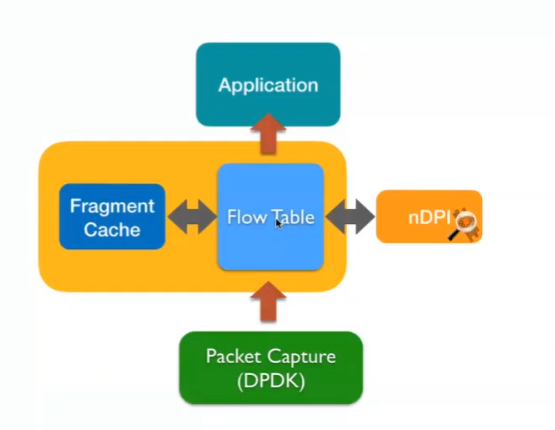
\includegraphics[scale=0.5]{ndpiarch.png}
\end{center}
\paragraph{Come usare} Applicazione cattura il pacchetto e mantiene il flusso di stato, nDPI si aspetta di ricevere il pacchetto.\\
Ogni dissettore è codificato in un differente \texttt{.c}, ognuno classifica il singolo protocollo, per modularità ed estensibilità.
\paragraph{Flow Lifecycle} La flowtable spesso esiste già. I flussi sono tenuti ordinati da qualcuno con una quintupletta+1 (VLAN, protocollo, IP/Porta, src/dst)\\
Applicazione va nella flowtable e cerca pacchetto precedente del flusso. Se esiste, prende l'informazione già memorizzata (cioè fin dove era rimasto nDPI su quel flusso), sennò si crea il nuovo flusso.\\
Se dopo un tot di iterazioni non riconosce ancora il protocollo lo cataloga come sconosciuto.\\
Il \textbf{riconoscimento} avviene \textbf{solo all'inizio del flusso}. Flussi mantenuti in hash sulla quintupletta.\\
Costo computazionale è sia numero pacchetti che numero di flussi
\paragraph{Traffic Classification Lifecycle} Basato sul tipo di traffico, dissectors applicati sequenzialmente iniziando con quello che più probabilmente matcherà (es HTTP dissector se traffico su TCP/80)\\
Ogni flusso mantiene lo stato per dissector non-matching per saltarli in futuro.\\
Analisi dura fino a match o dopo troppi tentativi (8 pacchetti solitamente)\\
Flusso è bidirezionale e corrisponde alla quintupletta IP+prot+porta+src+dest(+vlan)\ldots\\
Riconoscimento avviene solamente ad inizio del flusso.\\
nDPI funziona con i pacchetti IP.
\paragraph{Latenza applicativa di rete} Calcolata utilizzando il TCP durante l'handshaking, monitorando con un probe in un punto della rete ma non si può dire se cho messo pià temopio andata che ritorno.\\
Con sottrazioni trovo latenza rete e applicativa.
\begin{multicols}{2}
	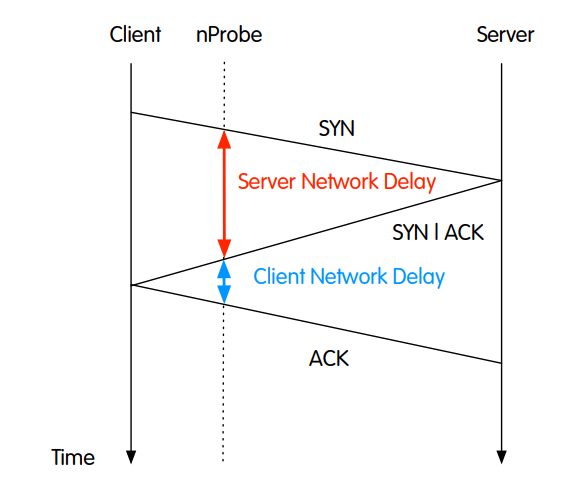
\includegraphics[scale=0.5]{latency1.png}\\
	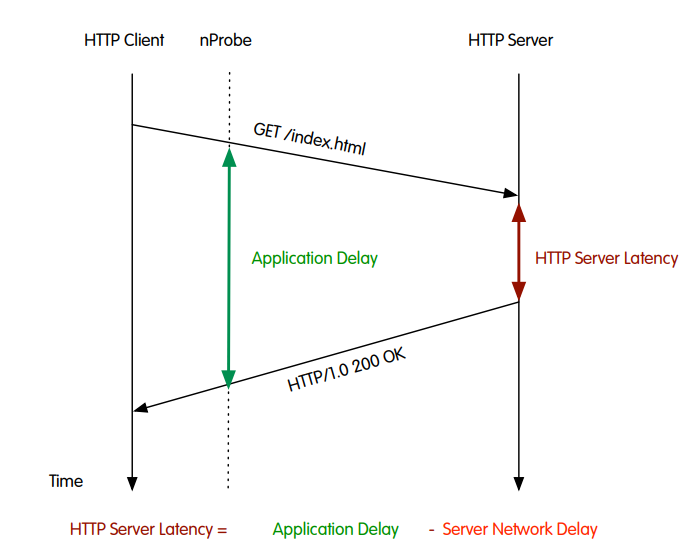
\includegraphics[scale=0.5]{latency2.png}
\end{multicols}
\paragraph{Throughput} Metrica misura quantità dati inviati su un link in un certo istante.\\
Quant'è il tempo? Tipicamente al secondo ma la durata del monitoring dev'essere maggiore, si guarda al secondo ma la durata dell'esperimento dev'essere maggiore. Throughout dice  indicazione idea di quanto è la banda disponibile.\\
Misura quantità di dati inviata in istante di tempo, \textbf{conservativa della banda disponibile} cioè misurando questo ho idea di quello che faccio effettivamente passare ma non della banda reale perché parte della banda la sto usando. Quindi \textbf{il throughput non è la banda}. Il throughput tipicamente cambia, la banda no. Inoltre è una misura orientata all'applicazione.
\paragraph{Goodput} Nei pacchetti c'è tanto overhead: ethernet, header IP, UDP\ldots fino al payload che è la \textbf{parte interessante}. Con il \textbf{goodput} si vede quanti dati effettivamente si spostano. Invece di misurare i byte inviati sul filo, vado a vedere i byte inviati di contenuto. Quando scarico un file di 1Mb ho mandato sul filo molto più di un 1Mb: header di ogni pacchetto, ACK per la connessione, RDY e FIN\ldots\\
Goodput mostra quanti dei dati transitati sono effettivamente usati per la connessione.
\paragraph{Latenza} Tempo che serve ad un pacchetto per andare \textbf{da sorgente a destinazione}, \textbf{monodirezionale}.\\
RTT (round trip time) è tempo di andata \textit{e ritorno}. La latenza non è RTT/2, ma la somma della latenza src2dst e latenza dst2src è l'RTT.
\paragraph{Jitter} Come cambia la latenza nel tempo: varianza dell'intrapacket delay su link monodirezionale.\\
Finché jitter è inferiore alla durata temporale del buffer lato ricezione, la comunicazione sarà ideale. Se io tengo buffer grande (1-2s) la voce la sento bene risolvendo il jitter, ma ho aumentata la latenza.\\
Questo perché i ritardi introdotti dalla rete non sono costanti.
\begin{center}
	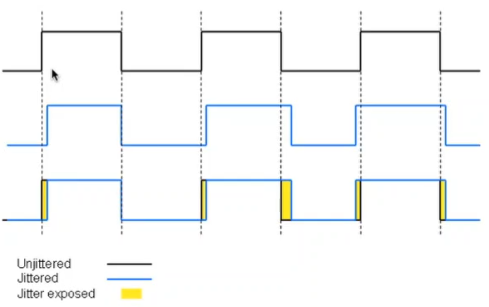
\includegraphics[scale=0.75]{jitter.png}
\end{center}
\paragraph{Bandwith} La banda è quella misura che stima più o meno quello che dovrebbe passare sul cavo. Viene calcolata: 
\begin{list}{}{}
	\item TC intervallo di misura, tipicamente 1s
	\item BC burst committed, n max bit/s che il network accetta di trasferire nel TC
	\item CIR committed information rate, banda garantita BC/TC
	\item BE burst excess, parte che trasporta in eccesso se ha disponibilità proverà a trasportarne di più 
	\item MaxR maximum data rate: (BC + BE)/TC = ((BC + BE)/BC)*CIR
\end{list}
\paragraph{Misure End-To-End} Nelle misure devo mettere in conto il tempo della mia applicazione per elaborare ed anche il ritardo di rete.\\
Performance di rete $\neq$ Performance app.\\
Bisogna fare attenzione rispetto alle misure per link, ad esempio perché traffico fa routing diverso andata-ritorno qudini rtt/2=latenza è in generale sbagliato. misure endtoend sono più vicine all'utente, si rapporta al server remoto non alla misura link link. Quella link link serve a noi per fare troubleshooting.\\
EndToEnd e LinkLink sono in relazione, endtoend dà se c'è problema che si scorpora sul link. EndtoEnd da informazione dal punto di vista utente, link dà info sul singolo link utiler per troubleshooting.
\paragraph{Approcci di monitoraggio} Sono multipli. fin'ora è una misura di tipo passivo: si cattura traffico, senza influenzare niente.\\
Nella misura attiva inietto del traffico e vedo la reazione della rete, ad es. un ping.\\
Ad es traceroute calcola latenza e da dove passa un certo tipo di traffico. Usa un trucco sul TTL: manda pacchetti che tornano indietro a causa del TTL basso.\\
\paragraph{Inline} Inline significa quando monitoriamo se tramite snmp connetto allo switch con lo stesso filo che snmp sta monitorando: \textbf{inline}.\\
Offline invece è monitoring tramite altra rete: reti sdoppiate, una per monitorare e una per i servizi. Vincolata dalla struttura della rete, a volte non possibile.\\\\
Quindi approcci attivi/passivi, inline/offline.
\section{Calcolo delle serie temporali}
Posso fare una misura mettendo una soglia assoluta, ma posso anche impostare queste soglie a seconda del comportamento della rete.\\
La media è la misura media, la deviazione standard è una misura "standard" di cosa è normale e di cosa è molto grande ($>$ media + devstd) o molto piccolo ($<$ media - devstd)
\paragraph{Percentile} Quando si prende una misurazione, es. quantità della banda, nel caso delle rete il 95esimo percentile è interessante. \textbf{Percentile} è valore sotto il quale ricade una certa percentuale di osservazioni.\\
Esempio: l'80esimo percentile è l'età in cui cade l'80\% della popolazione.\\
Perché importante? Se devo parlare ad esempio della banda, posso calcolare economicamente parlando per vedere se quella banda è utilizzata, o per vedere se la banda che metto a disposizione è utilizzata. Quando arriva il momento di fare un upgrade, ad esempio? Oppure anche usabile per far pagare delle penalty.\\
Il 95esimo percentile di una rete è la soglia sotto cui sono stato per il 95\% del tempo.\\
Calcolo: data una serie di valori, si definisce il percentile (es. 80), si ordina la serie dal passo all'alto, calcolo indice che corrisponde al percentie (len(serie)*(percentile/100)), prendo l'indice intero (es int(index + 0.5))\\
Percentile = serie\_ordinata[indiceintero-1]
\paragraph{Quartile} \begin{list}{}{Definiti così:}
		\item $Q_1$ è il 25esimo percentile
		\item $Q_2$ è il 50esimo percentile
		\item $Q_3$ è il 75esimo percentile
\end{list}
\begin{center}
	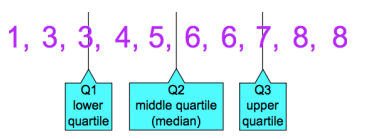
\includegraphics[scale=1]{quartile.png}
\end{center}
\subparagraph{Outlier} Ciò che devia un sacco dallo standard.\\
Punti che discostano tantissimo rispetto all'average. Si usa l'IQR (InterQuartile Range): $Q_3 - Q_1$
\begin{center}
	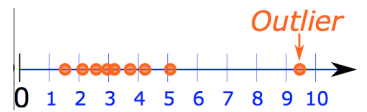
\includegraphics[scale=1]{outlier.png}
\end{center}
\begin{list}{}{In statistica, un valore è un outlier quando cado fuori da}
	\item Lower Fence: $Q_1 - 1.5\times IQR$
	\item Upper Fence: $Q_3 + 1.5\times IQR$
\end{list}
Si usano per trovare valori anomali, come errori di misura o sperimentali, o distribuzioni "heavy tailed", cioè che vanno a zero molto lentamente poiché una o più valori molto grandi hanno effetto sulla statistica.
\paragraph{Calcolo del jitter} \texttt{jitter = sum(|x(i) - x(i-1)|) / (n-1)}\\
Se il jitter è nell'ordine di grandezza del valore allora la situazione è drammatica. Jitter basso: valore costante. Jitter alto: valore cambia spesso nel tempo.
\subsection{Timeseries, Forecast, Anomaly Detection}
Negli RRD c'erano dei valori $\alpha$, $\beta$, $\gamma$ che avevamo detto di lasciare quelli di default. Sono serie temporali su cui vogliamo fare delle previsioni, che ci forniscono le anomalie. Quand'è che una cosa è anormale? Quando ho il concetto di normalità. Ad esempio, una soglia. Quindi come trovare le condizioni tali in cui il sistema che sto guardando si comporta stranamente?\\
\begin{list}{}{\textbf{Definizioni}:}
	\item \textbf{Serie}: sequenza ordinata di numeri, non sorted ma con indici
	\item \textbf{Ordine}: indice di un numero in una serie
	\item \textbf{Serie temporale}: serie di punti ordinati temporalmente
	\item \textbf{Osservazione}: valore numerico osservato (nella realtà) in un momento specifico
	\item \textbf{Previsione}: stima di un valore atteso (che non sappiamo ancora) in un momento specifico (\textit{alle 12 quanto traffico farò?})
	\item \textbf{Anomalia} quando la \textbf{previsione} scosta dall'\textbf{osservazione}
	\item \textbf{Forecast error}: differenza positiva/negativa nell'osservazione rispetto alla previsione. Solitamente l'errore è riportato come quadrato per avere sempre numero positivo.
	\item \textbf{SSE}: la somma degli errori quadrati (\textbf{sum of squared errors}) di una serie \texttt{sum((osservazione$_i$ - previsione$_i$)$^2$)}\\
	Idealmente deve essere 0, o comunque basso
	\item Dato $y$, $\overline{y}_{x+1}$ è la predizione di $y$ al tempo $x+1$
	\item \textbf{Simple Average}: media di tutti i punti della serie
	\item \textbf{Moving Average}: media degli ultimi $n$ punti
	\item \textbf{Weighted Moving Average}: come la media mobile ma con i valori pesati (tipicamente pesando di più i valori più recenti)
\end{list}
\textbf{Anomalia} quando \textbf{la predizione và in conflitto con l'osservazione}.
\paragraph{Predirre il futuro}
\begin{center}
	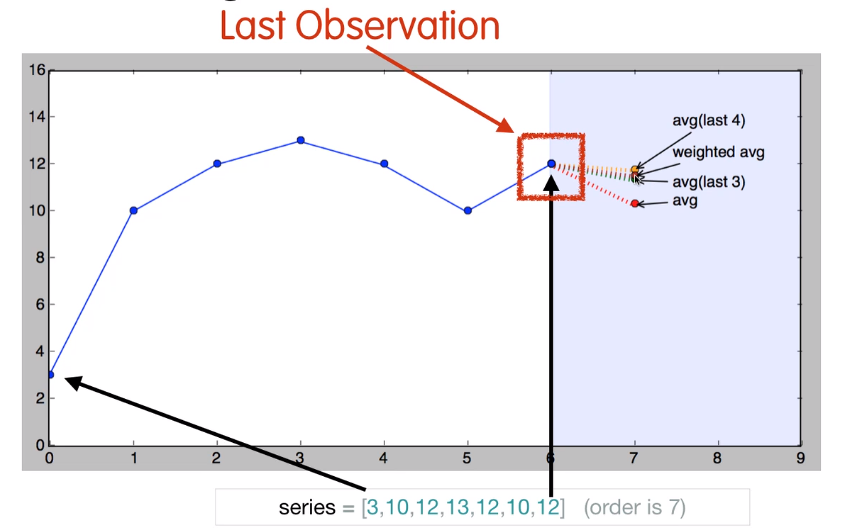
\includegraphics[scale=0.7]{averageforectast.png}
\end{center}
\subparagraph{Single Exponential Smoothing}
$\overline{y}_x = \alpha\cdot y_x + (1 - \alpha) \cdot \overline{y}_{x-1}$\\
$\alpha$ è un fattore di \textbf{ammorbidimento} o \textbf{memory decay rate}, più alto è più tengo presente gli ultimi valori e meno tengo presente i vecchi.\\
$\overline{y}_x$ è chiamato livello $l_x$
\subparagraph{Double Exponential Smoothing}
Trend $b$ su una serie temporale, fra due punti è $y_x - y_{x-1}$
$b_x$ = $\beta\cdot(l_x - l_{x-1})$\ldots\\
Con $\beta$ non prendo solo la media ma tengo conto anche del trend, così da avere previsioni più accurate. Quindi alla previsione si aggiunge $b_x$
\begin{list}{}{}
	\item Livello $l_x = \alpha\cdot y_x + (1-\alpha)\cdot(l_{x-1}+b_{x-1})$
	\item Trend $b_x = \beta\cdot(l_x - l_{x-1}) + (a-\beta)\cdot b_{x-1}$
	\item Previsione $\overline{y}_{x+1} = l_x + b_x$
\end{list}
\begin{center}
	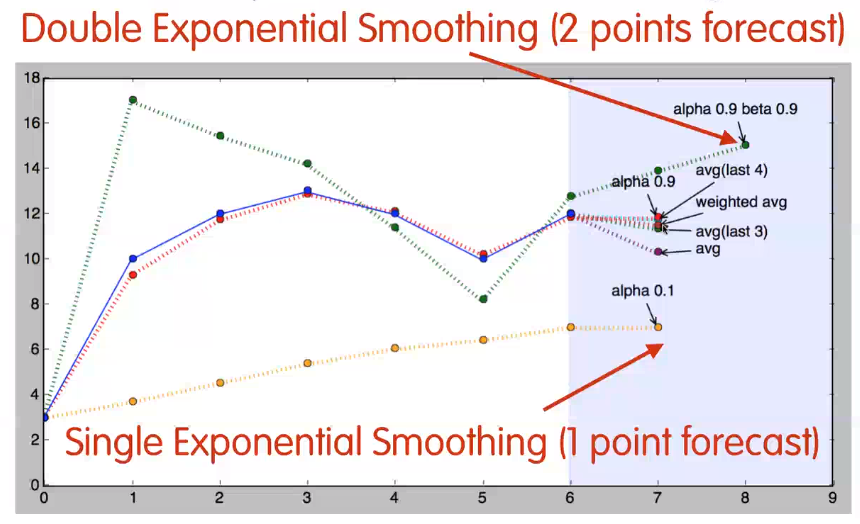
\includegraphics[scale=0.7]{doubexpsmo.png}
\end{center}

\paragraph{Holt-Winters Method} Anche detto \textbf{Triple Exponential Smoothing}\\
Nel double exponential smoothing manca il concetto di \textbf{stagione}: quando una serie è ripetitiva a intervalli regolari si dice \textbf{stagionale}.\\
Lunghezza della stagione: numero dei data point in una stagione.\\
Componente stagionale: deviazione da level+trend del double exponential che si ripete all'interno della stagione.\\
$\gamma$ fornisce il concetto di stagionalità. Serve il modulo della durata della stagione, perché è in loop. Inoltre con H-W posso \textbf{predire un numero arbitrario di punti}. valori più grandi danno previsione meno conservativa. $\alpha, \beta, \gamma$ si assegnano tramite il \textbf{fitting}.
\begin{list}{}{}
	\item Livello $l_x = \alpha\cdot y_x + (1-\alpha)\cdot(l_{x-1} + b_{x-1})$
	\item Trend $b_x = \beta\cdot (l_x - l_{x-1}) + (1-\beta)\cdot b_{x-1}$
	\item Stagionale $s_x = \gamma\cdot (y_x - l_x) + (1-\gamma)\cdot s_{x-L}$
	\item Previsione $\overline{y}_{x+m} = l_x + m\cdot b_x + s_{x - L + 1 + ((m-1)\textsl{ mod }L)}$
\end{list}
Per prevedere un numero arbitrario $m$ di punti.\\
$\alpha,\beta$ e $\gamma$ sono i parametri di adattamento per l'algoritmo, con $0<\alpha,\beta,\gamma < 1$. Valori più grandi rendono l'algoritmo in grado di adattarsi più rapidamente e fanno in modo che le previsioni riflettano di più i cambiamenti recenti nella time serie. Valori più piccoli, invece, rendono l'algoritmo più lento all'adattamento, rendendo più importanti i valori passati nell'history.\\
I valori per $\alpha,\beta$ e $\gamma$ possono essere determinati provando a determinare la più piccola SSE (Sum of Squared Errors) in un processo iterativo chiamato fitting (simile al ML).
\subparagraph{Deviazione in H-W} La deviazione può essere identificata quando l'osservazione cade al di fuori delle fasce di confidenza minima e massima per un dato punto.\\
$d_t = \gamma\cdot |y_t - \overline{y}_t| + (1 - \gamma)\cdot d_{t-m}$\\
Fasce di confidenza con $\delta$ tra 2 e 3:
\begin{list}{}{}
	\item Superiore: $\overline{y}_t - \delta\cdot d_{t-m}$
	\item Inferiore: $\overline{y}_t + \delta\cdot d_{t-m}$
\end{list}

\chapter{Remote Monitoring}
\textbf{Analisi rete remota rispetto dove siamo noi}.\\
Importante perché tutta la parte interessata dalle informazioni sta alla periferia di internet (\textbf{edge computing}), inoltre è anche "forzato" dalle parti wireless che stanno diventando predominanti. Dal core ci passa si traffico ma è sempre minore. Il core diventa meno importante perché comunicaz in perferia.\\
Diventa necessario \ldots Inote tipi traffici che nascono e muoiono in periferia senza passare dal core.\\
Il problema è andare a spillare il traffico remoto, vedere il traffico che fluisce in questa rete. Nn sempre banale perché magari necessario modificare la rete. Quindi attenzione alla topologia, e attenzione ai tap di rete usati percHé hanno limitazioni importanti.\\
Anche le funzionalità di monitoraggio degli apparati di rete comuni sono limitate, spesso il massimo che posso vedere sono i byte totali, ip assegnati\ldots\\
Spesso i costi per sistemi di monitoring sono importanti.\\
Misura in remoto tramite snmp nasce subito dopo mibv2. con snmp misuro quanto ma non posso fare misure pià complicate, e non posso assegnare soglie e in base mandare allarme ma misurare in continuazione e fare i nostri calcolo.\\
MIB RMON (MIB SNMP), risolve problema monitoraggio remoto. Consente di gestire disservizi. Inserisce un minimo di logica per generare allarmi.
\section{RMON} Cosa fà? Primo passaggio da monitoraggio snmp a monitoraggio a pacchetti.\\
Vedo traffico di rete remoto e metto una sonda remota.\\
\textbf{RMON è un MIB SNMP}.
\subparagraph{RMON vs SNMP} SNMP controlla e configura un probe, solitamente con GUI. SNMP esegue la \textbf{richiesta periodica} (polling). L'azione è eseguita dal manager.\\
RMON sposta un po' della logica nell'apparato, che raccoglie da sé stat e impostare allarmi direttamente sull'apparato.
\begin{list}{}{\textbf{Gruppi RMON}}
	\item Statistics: vedo info che SNMP non dà precisamente, es pacchetti droppati
	\item History: dati i contatori (es. quante volte una porta cambia stato) consente di non andare sullo switch e leggere e scrivermeli ma chiedere la storia recente del contatore. Memoria piccola, 3-5-10 misure, poche. RMON legge un po' nel passato, SNMP legge sempre e solo in real-time
	\item Alarm: 
	\item Host: a livello di host quali traffici per un certo host, es. byte in out per certo host.
	\item HostTopN: per i top N host quanto traffico fanno, quale porta più occupata. Se c'è connesso un PC è il colpevole, ma se ce ne sono N non mi è chiaro. Con HostTopN analizzo traffico della porta e trovo N computer che fanno più traffico\ldots
	\item Matrix: mostra comunicazioni tra indirizzi
	\item Filters: per filtrare il traffico di rete
	\item Packet capture: per catturare un pacchetto una volta che è passato attraverso il canale
	\item Events: per generare eventi sotto certe condizioni
\end{list}
\paragraph{Statistiche ethernet RMON}
\begin{list}{}{Informazioni di basso livello}
	\item Pacchetti: unicast, multicast e broadcast.
	\item Eventi di drop: pacchetti droppati per sovraccarico linea/porta
	\item Frammenti: quanti frammenti sono passati. Ci sono attacchi basati sui frammenti.
	\item Jabbers: pacchetti ricevuti più lunghi di 1518 ottetti e con errori di allineamento
	\item Oversized packets: pacchetti più lunghi di 1518 ottetti ma altrimenti ben formati
\end{list}
C'è anche una formula per capire quanto è usata una porta di rete (100x((packets x 160)+(octets x 8)))/(portspeed x timeinsec)
\paragraph{Allarmi} Impostare soglie su contatori di RMON, soglie di due tipi: rising e falling. Quando troppo alta (rising) o bassa (falling) posso effettuare operazioni.\\
Es troppo traffico se utilizzo sup a 80\% manda allarme.
\paragraph{Case Study} \ldots RMON va a mappare ogni quanto misuro dati, valori di soglia
\paragraph{NBAR} Statistiche di traffico stile RMON
\section{RTFM} Real-Time Flow Measurement
\begin{multicols}{2}
Cambio di architettura per andare oltre l'architettura SNMP
\begin{list}{}{}
	\item Meter: colui che misura, il contatore. Và messo dove passa il traffico
	\item Reader: parla col meter e tira fuori i suoi dati. Deve essere "vicino" al meter, ma non è dentro
	\item Manager: gestisce configurazione di meter e reader e che chiede i dati. Implementato in SNMP
	\item Applicazione: fa i grafici, configura il manager\ldots
\end{list}
\begin{center}
	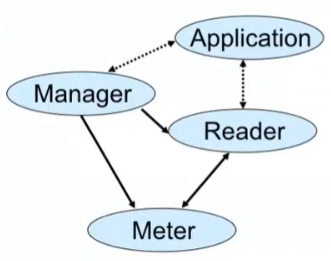
\includegraphics[scale=0.5]{rtfm.png}
\end{center}
\end{multicols}
\section{Monitoraggio a flussi}
Nel caso di SNMP agent (dove passa traffico) e manager (query all'agent). Nel caso di un problema, agent avverte manager tramite trap (cambio di stato, o superamento soglia in caso di RMON).\\
Agent snmp non è libero di monitorare tutto, si limita al MIB.\\
Nei flussi prendo traffico di rete, lo metto insieme in base a caratt (es protocollo, stesso ip:porta sorg, stesso ip:porta dest = quintupletta)\\
Non configuro il flusso. Nel caso di NetFlow la device stessa dove passa il traffico di rete (es router) prende e spara verso collezionatore (manager) le informazioni da monitorare. In questo caso quindi i flussi sono prodotti ed emessi verso colui che deve riceverli.\\
No concetto allarme ne abilità per agents di fare alcunché: tutta la logica è nel collezionatore.\\
Strumentazione del probe è fatta offline.\\
Probe sono posizionati dove fluisce il traffico, tipicamente nel router.\\
\textbf{Cosa si misura?} Dove viene scambiato il traffico organizzato per gruppi autonomi, IP\ldots\\
A livello applicativo quanto traffico in base a porta o protocollo\\
Quali servizi, livelli di traffico\ldots anche rintracciare virus di rete fino agli host.\\
Con i flussi non si riesce a misurare traffico nonIP, informazioni livello 2 (stato delle interfacce), traffico flitrato (firewall), statistiche per-link (livello di utilizzo, congestione, perdita\ldots), statistiche per applicazioni (es latenza, risposte positive/negative, errori di protocollo).
\paragraph{Flusso}: insieme di pacchetti accumunati da una stessa quintupletta. Flussi sia unidirezionali che bidirezionali. Calcolati dal probe (era: agent) che guarda traffico che passa attraverso e lo misura. Flusso creato quando vedo il primo pacchetto del flusso, probe sta fermo.\\
Massima durata flusso regardless lo stato della connessione: termino flusso o quando dura troppo o quando non c'è traffico per un po' di tempo.\\
Contenuti del flusso: peers (src e dst), contatori (packets, bytes, tempo), info routing (sistema autonomo, netmask, interfaces).\\
Possono essere uni e bidirezionali. Due flussi unidirezionali opposti sono equiv a uno bidirezionale. Flussi bid possono contenere altre info come rtt o comportamento tcp.\\
\textbf{Problemi vari}\\
\begin{list}{}{Overhead vs accuratezza}
	\item + misure + dati
	\item + aggregazione flussi - granularità
	\item overhead su router, switc e endhosts
\end{list}
\begin{list}{}{Security vs data sharing}
	\item flussi devono andare ai collezionatori su cammini protetti
	\item privacy va rispettata
	\item misure di traffico devono essere mantenute protette per non rivelare informazioni di rete importanti a terze parti
\end{list}

\chapter{ScaPy}
Manipolazione di pacchetti in maniera semplice. Con Pcap si legge e invia, ma gestisce i pacchetti raw e non permette di manipolarli, funge da specie di socket. Wireshark è molto utile ma è un tool a sé state, ma se serve fare cose in batch non è molto utile. Wireshark può essere collegato tramite API a PyShark, ma è sola lettura. ScaPy permette sia di inviare che di ricevere.
\paragraph{Modulo} ScaPy è un modulo Python.\\
Cosa ci possiamo fare? \begin{list}{}{}
	\item \textbf{Manipolazione dei pacchetti}\\
	Ha un operatore particolare, \texttt{/} che permette di creare un pacchetto, esempio: \texttt{packet = IP() / TCP()} che crea un pacchetto IP e sopra ci mette una parte TCP. Senza i parametri lo crea con opzioni di default (es IPv4) e non bisogna preoccuparci granché dei campi non riempiti, possiamo spedirlo (anche se non va da nessuna parte perché non ha indirizzo di destinazione).\\
	Con \texttt{ls(IP, verbose=True)} stampa i vari campi, con tipo e valore. Più o meno è la stessa informazione vista con Wireshark e Tshark.\\
	Volendo posso stampare un campo voluto, ad esempio con \texttt{print(p[IP].src)}.\\
	\texttt{summary()} stampa tutti i campi del pacchetto.
	\item \textbf{Interagire con la rete}\\
	Permette di inviare e ricevere i pacchetti, oltre a crearli. La funzione per inviare traffico è \texttt{srl()}, ad esempio\\\texttt{r = srl(IP(dst="8.8.8.8") / UDP() / DNS(qd=DNSQR()))}.\\
	\texttt{srl()} riceve anche la risposta, che nell'esempio sarà memorizzata in \texttt{r}, che posso leggere ad esempio con \texttt{r[DNS].an}.\\
	\texttt{srp()} invece consente anche di specificare la parte ethernet. Spedisce una lista di frame e ritorna due variabili
	\begin{list}{}{}
		\item \texttt{r}, lista di query e risposte
		\item \texttt{u}, lista di pacchetti non risposti
	\end{list}
	\item \textbf{Pcap}\\
	Possiamo leggere e scrivere un file pcap, con \texttt{wrpcap("file.pcap", r)} e \texttt{rdpcap("file.pcap")}\ldots\\
	Con \texttt{command()} su un pacchetto pcap, ritorna il comando da fare con ScaPy per ricreare un pacchetto di pcap.
	\item \textbf{Sniffing}\\
	Con il comando \texttt{sniff()}, applicando filtri, funzioni\ldots\\
	\item \textbf{ARP}\\
	Con \texttt{arping("192.168.1.0/24")} per mandare richieste ARP sulla rete specificata. La differenza con ICMP è che il ping classico può essere ignorato. Con ICMP quando c'è risposta la macchina è attiva, quando non c'è non si può sapere.
	\item \textbf{AnsweringMachine}\\
	Permette di gestire le risposte, un esempio è avviarla in monitoring su un'interfaccia. 
\end{list}
\chapter{Flussi}
\paragraph{Flussi unidirezionali con IP src/dst come key}
\paragraph{Flussi unidirezionali con IP, Porta e protocollo come key} Avrò più flussi perché distinguo anche i protocolli usati e le porte, quindi ho maggiore informazione sul traffico.
\paragraph{NetFlow} Architettura a flussi, prima coniata da Cisco. Funziona diversamente da ciò che si è visto fin'ora. Abbiamo un router con un probe (sonda di rete, traduce pacchetti in flussi). La funzionalità di misura è secondaria (il router deve andare bene), ma catalogare i flussi richiede memoria. Router calcola i valori con il probe ma non ha capacità di memorizzazione: manda verso Flow Collector (un pc con un software apposito). Il collezionatore riceve flussi e fa qualcosa: es. manda dati a interfaccia web.\\
C'è anche problema se si monitora rete abbastanza grande. Si possono mettere più collezionatori che collaborano fra loro, ognuno attaccato ad un endpoint (router verso l'esterno) della rete.
\paragraph{Spazio} Lo spazio richiesto dipende dal traffico. Qualche valore solito:
\begin{list}{}{}
	\item 67320 ottetti/flusso, 92 pacchetti/flusso
	\item Router occupato: 367GB traffico al giorno, 548000000 pacchetti al giorno, cioè 5900000 flussi al giorno
	\item %TODO
\end{list}
\begin{multicols}{2}
\begin{center}
	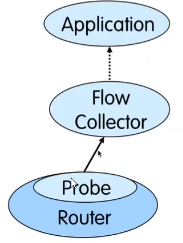
\includegraphics[scale=0.5]{netflow.png}
\end{center}
\columnbreak
\paragraph{NetFlow} Flussi unidirezionali fino a v8, bidirezionali dal v9. La più comune è v5, l'ultima è v9.\\
Analisi solo del traffico inbound e IP (non su tutte le piattaforme). IPv4 unicast e multicast. IPv6 solo su v9. La v9 è aperta, cioè integrabile con moduli personalizzati.\\
Protocollo aperto definito da Cisco e supportato su IOS e CatIOS e su altre piattaforme Cisco.\\
Ogni versione ha un formato di pacchetti: fino alla 8 era chiuso, dalla v9 è dinamico e aperto a estensioni.\\
Numeri di sequenza: v1 non ha numeri di sequenza, fino alla 8 numeri di sequenza per flusso e dalla 9 numeri di sequenza per pacchetto (non flusso)\\
Qualche versione è specifica per alcune piattaforme di Cisco.
\end{multicols}
\begin{center}
	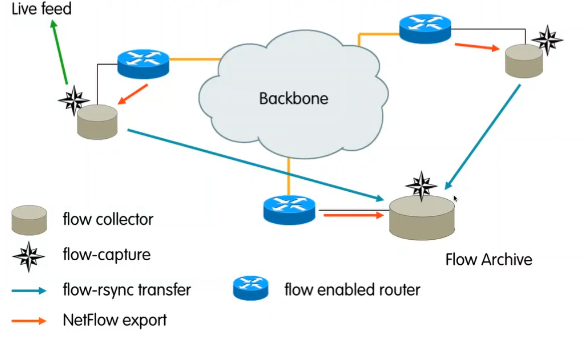
\includegraphics[scale=0.75]{netflowarch.png}\\
	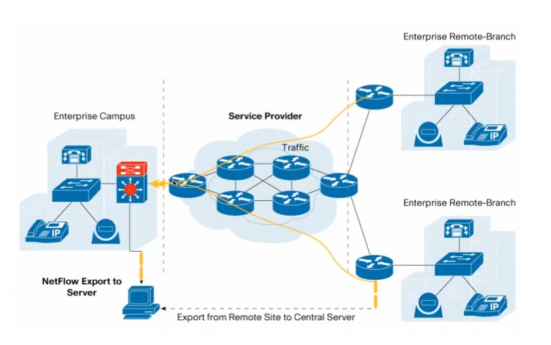
\includegraphics[scale=0.75]{netflowarch2.png}
\end{center}
\begin{multicols}{2}
\paragraph{Usare i flussi} Cosa c'è dentro un flusso? Questa domanda risponde anche a cosa ci faccio con essi.
\begin{list}{}{Nella parte di chiave: la quintupletta}
	\item Protocollo
	\item IP src/dst
	\item Porta src/dst
\end{list}
\begin{list}{}{Altre info}
	\item QoS: Flag TCP, tipo protocollo e tipo di servizio
	\item Porta: indice di porta in e out
	\item Info di routing: next hop, da/verso quale AS\ldots
	\item Contatori: di byte e di paccketti
	\item Tempo: sysuptime start/end
\end{list}
\columnbreak
\begin{center}
	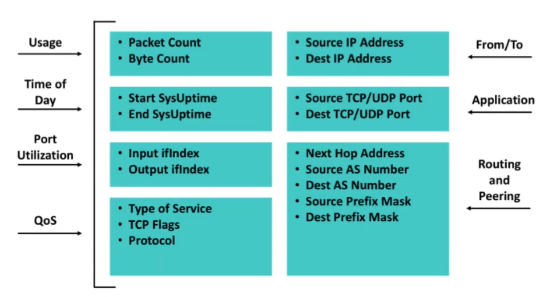
\includegraphics[scale=0.6]{useflows.png}
\end{center}
\end{multicols}
\begin{multicols}{2}
\begin{center}
	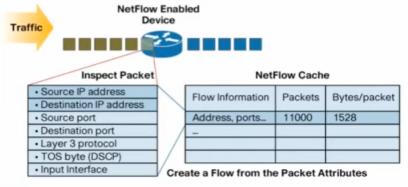
\includegraphics[scale=0.75]{flowcache.png}
\end{center}
\columnbreak
\paragraph{Nascita e morte di un flusso} Siamo a livello 3. Il traffico deve entrare e uscire dal router, quindi interf ingr e usc: il traffico è esaminato, cioè passato al probe. Posso mettere nel pc di casa un software per sniffing, ma nel router i pacchetti passano attraverso di lui. Probe prende dati e li raggruppa, li gestisce. Si tiene una cache dei flussi attivi. Appena c'è pacchetto non conosciuto la popola.\\Al suo interno ha sistema ispezione pacchetti. In cache c'è una sorta di hashtable, come chiave ho ip porte\ldots, come valore ho \textit{almeno} i byte e i pacchetti.
\end{multicols}

Terminano quando:
\begin{list}{}{}
	\item La comunicazione di rete termina (es: FIN)
	\item Dura troppo (default 30m)
	\item Non attivo da troppo (default 15s)
	\item Cache piena e necessario purge (è limitata, non è raro non poter gestire tutti i flussi)
\end{list}
Perché taglio quando il flusso dura troppo? Sennò manderei i dati tutti alla fine, con picchi di traffico, e sballerebbe le misura.
\paragraph{Pacchetti NetFlow} Header comune rispetto alle varie versioni. A seconda della versione c'è un campo che specifica il numero di record $N$. $N$ è determinato dalla dimensione massima del payload UDP (circa 1480 byte), $N=30$ per v5. Nessuna frammentazione.\\
Header contiene:\begin{list}{}{}
	\item \textbf{version} es: 5
	\item \textbf{count} (numero di record nel payload)
	\item \textbf{sysuptime} del router (da quanto è acceso)
	\item \textbf{unix\_secs} (epoca del flusso, secondi da 0000 UTC 1970)
	\item \textbf{unix\_nsecs}
	\item \textbf{flow\_sequence} (numero di flussi inviati, per sapere se collezionatore si è perso qualcosa non sa cosa ma sa di aver perso qualcosa)
	\item \textbf{engine\_type} per caratterizzare tramite info su chi ha generato i dati
	\item \textbf{engine\_id} numero di slot per l'engine
\end{list}
Flusso contiene:
\begin{multicols}{2}
 \begin{list}{}{}
	\item \textbf{srcaddr} ipv4
	\item \textbf{dstaddr} ipv4
	\item \textbf{nexthop} (per sapere come viene routato traffico dentro il pc: 
	\item \textbf{input} indice di interfaccia snmp
	\item \textbf{output} indice di interfaccia snmp
	\item \textbf{dPkts} numero pacchetti
	\item \textbf{dOctets} numero ottetti
	\item \textbf{First} sysuptime dell'inizio del flusso
	\item \textbf{Last} sysuptime dell'ultimo pacchetto
	\item \textbf{srcport} TCP/UDP porta origine
	\item \textbf{dstport} TCP/UDP porta destinazione
	\item \textbf{pad1} padding
	\item \textbf{tcp\_flags} or cumulativo dei flag tcp
	\item \textbf{prot} protocollo ip (6=TCP, 17=UDP\ldots)
	\item \textbf{tos} type-of-service
	\item \textbf{src\_as} as origine
	\item \textbf{dst\_as} as destinazione
	\item \textbf{src\_mask} bitmask source route
	\item \textbf{dst\_mask} bitmask dest route
	\item \textbf{pad2} padding
 \end{list}
\end{multicols}
\paragraph{Pacchetto NetFlow} In SNMP dati letti tramite polling (eccettuate le trap). Cambi di stato SNMP sono pochi, agent SNMP non fa attesa attiva ma è S.O. stesso a comunicare a SNMP quando cambia qualcosa. Es: Inotify (\texttt{wikipedia.org/wiki/Inotify}, notifica cambiamenti a file/cartelle) o netlink (\texttt{wikipedia.org/wiki/Netlink}, notifica cambiamenti su rete e interfacce) su Linux.\\
In NetFlow però siamo obbligati ad analizzare attivamente ogni pacchetto che passa. Inoltre buffering limitato, quindi pacchetti vanno gestiti subito. Inoltre la quantità di flussi da esportare dipende molto dal tipo di traffico. Può esserci un solo flusso su 10 gigabit, ma posso avere decide di flussi su 7 megabit.\\
Il traffico conteggiato da NetFlow è inferiore da quello che verrebbe contato da SNMP. SNMP ne cattura di più in caso ci sia traffico multicast/broadcast. Inoltre SNMP è livello 2 (comprende il payload del livello frame) ma NetFlow è livello 3, non conta il traffico di livello frame. Ad esempio ARP non lo vedo in NetFlow perché è di livello 2.\\
\textbf{NetFlow conta solo il traffico che passa \textit{attraverso} il router, cioè che viene instradato.}
\paragraph{Perché serve NetFlow v9?} La v5 ha solo IPv4, poche informazioni (pacchetti e byte). Ogni volta che si deve aggiungere qualcosa bisogna rifare il formato, aggiornare software\ldots\\
In v9 risolvono problema della flessibilità: flussi mandati con un template che indica i campi. Inoltre supporta il livello 2, traffico VLAN e altri tipi di incapuslamento come MPLS, oltre che IPv6.
\subparagraph{Template} Mandato prima dei flussi, così da specificare al collezionatore in che modo interpretare i dati ricevuti. Specifica una maniera di mappare le info relative al flusso.\\
Vengono mandati periodicamente.
\paragraph{Sampling} Per ridurre il carico sulla macchina introduco il sampling: non analizzo ogni pacchetto, ma ad esempio uno su 10. Questo introduce un errore, sia sul conteggio dei byte che sulle informazioni trovate. Sampling da usare solamente in situazioni particolari.\\
Si parla di \textbf{packet sampling}, ma si può fare anche \textbf{flow sampling} (esempio: esportarne uno su 10). Questo per ridurre il traffico sul collezionatore.
\paragraph{Principi del v9} Modello push probe verso collezionatore come in v5\\
Manda template regolarmente (ogni tot flussi, ogni tot secondi)\\
Indipendente dal protocollo sottostante (UDP/TCP)\\
Può andare sia template che record in una export\\
Può mischiare le informazioni sui flussi nel singolo record.\\
Posso inserire nuovi campi oltre counting di pacchetti e byte: contenuto, velocità\ldots\\
Si aggiorna \textit{ogni tanto}, all'esportazione del flusso (tipicamente scadenza timeout)\\
Salta 24Byte perché parte da livello 3.
\paragraph{Message Broker} Prende messaggi e li smista a seconda di caratteristiche a chi si è sottoscritto, volendo anche riformandoli in formati diversi.
\subparagraph{Configurazione Cisco IOS} Configurato su ogni interfaccia, specificando versione e IP del collezionatore. Specifico sampling rate, durata massima e aggregazione (\\
Si abilitano flussi basandoli sull'interfaccia.
\subparagraph{Configurazione Juniper JunOS} Si appoggia al firewall, quando pacchetti attraversano router (eventualmente non filtrante). Router divisi in data/switching plane (hw) e control plane (sw). Sorta di loopback interno per analisi traffico, per portarlo da data a control plane. Juniper usa questa interfaccia per portare pacchetti in parte di controllo, limitata a 7000 pacchetti al secondo per evitare sovraccarico. Nello spazio utente c'è il probe che calcola i flussi ed esporta.
\paragraph{NetFlow generico: IPFIX} A inizio 2000 perché NetFlow è di Cisco\\
\textbf{IPFIX} definito dalla IETF.\\
Basato su NetFlow v9, abilità di definire nuovi campi del flusso attraverso un formato standard (OID, Object Identifier). Dopo aver definito il "PEN?" specifico OID univoci per me e in generale.\\
Protocollo di trasporto (SCTP, Stream Control Transport Protocol) orientato allo stream, connection-oriented, vincoli rilassati così da non perdere eventualmente troppo tempo a riempire il pacchetto. Opzionalmente supporta TCP/UDP.\\
Attualmente: bozza di specifica del protocollo.\\
\textbf{Fondamentalmente}, IPFIX = NetFlow v9 su SCTP con qualche differenza extra.
\paragraph{Aggregazione flussi} Flussi raw ok esporto e via. Spesso dobbiamo rispondere a domande diverse: quanto traffico certo protocollo? Quando verso Google?\\
Una volta che ho i flussi dentro il router posso esportarli raw o aggregarli: accorpare fra loro flussi a seconda di criteri stabiliti (es: IP, maschero le altre colonne come se non ci fossero ad esempio con valore fittizio 0 e sommando eventuali contatori). \textbf{Risparmio spazio e trasmissione}. Perdo informazione, non posso separare flussi aggregati.\\
Permette di trovare forme tipiche per rispondere a domande tipo: porte più usate, chi parla con chi\ldots\\
Una volta aggregati i dati, se fatta bene, risparmio molto spazio nella cache.
\paragraph{Filtraggio flussi} Scartare flussi basandosi su criteri: furata, src/dest, porte\ldots\\
Magari esportare solo unidirezionali. Diverso da aggregazione, possono coesistere e solitamente filtraggio applicato prima dell'aggregazione.
\paragraph{Esempi di intrusione} Flussi con pacchetti o ottetti eccessivi conteggio\\Src con tante destinazioni (host scanning) o con tante porte dest su stesso host (port scanning)
\subsection{sFlow}
Flow da non associare a NetFlow. NetFlow: insieme di pacchetti con caratteristiche in comune (a meno di aggregazione). NetFlow nasce per girare intralan, sui router per traffico che passa attraverso. Con probe software, ma anche hardware.\\
NetFlow è nato soprattutto per la parte geografica, non per la LAN. Se voglio sapere quello che succede in rete, il traffico non passa dal router: non vedrò con NetFlow ciò che passa in casa.\\
8 porte gigabit: 16 gigabit di traffico (8 gigabit andata e 8 gigabit ritorno). Diventa complicato analizzarlo.\\
Devo \textbf{deduplicare}: dividerlo a metà per le due direzioni.\\
Su una rete reale il traffico da analizzare è troppo: costerebbe di più l'infrastruttura. Inoltre sonde software richiedono lavoro: versioni diverse, librerie\ldots e non è detto che si possa installare probe.\\
Entra in campo sFlow. Ci si orienta verso di esso perché aumentando i problemi aumentano i costi. Aumentando porte devo aumentare potenza e memorizzazione. Ma devo partire dal perché voglio analizzare: visibilità di rete per sapere se ci sono problemi, come stanno andando le cose. La domanda è la visibilità. sFlow non pretende di vedere tutto sempre, non pretende di essere veloce quanto la rete, si analizza 1 pacchetto ogni $x$ (\textbf{Campionamento}: $x$ random, non fisso, sennò rischio di sincronizzarmi con traffico periodico e vedere sempre il solito), più pacchetti si analizzano più preciso sono ma se la rete è troppo veloce si campiona di più.\\
\textbf{Perdita controllata}.
\paragraph{Architettura} Probe campiona traffico, pacchetti campionati mandati all'sFlow collector in formato sFlow, periodicamente il probe manda al collezionatore le statistiche SNMP MIB-II all'interno dei pacchetti sFlow. Pacchetti usati per scalare il traffico. Il sampling è fatto per porta, per avere una visibilità per porta.\\
La differenza è che \textbf{il probe manda il pacchetto ogni $n$ con l'header sFlow e lo manda al collezionatore, senza analizzarlo}. Ci permette di andare veloci.\\\\
\texttt{RFC 3176}, definisce formato pacchetti (UDP, non SNMP) e un MIB SNMP per accedere i dati. Architettura simile a NetFlow: probe manda \textbf{pacchetti} al collezionatore.\\
probe fondamentalmente sniffer che cattura 1 ogni $x$ pacchetti (tipicamente $x = 400$ e incapsula con info sFlow.\\
Errore statistico $\leq 196\cdot\sqrt{\frac{1}{\textsl{numero dei sample}}}$\\
Scalabile (aumento il rateo di sampling).\\\\
sFlow $\neq$ NetFlow\\
Flussi sFlow e flussi NetFlow \textbf{non hanno niente in comune}. In sFlow un campione è un flusso, in NetFlow un flusso è una quintupla con contatori.\\
Oltre a vedere il pacchetto può mostrare anche info sul contesto agendo sullo switch\\
AS source e destination relative ad ip src/dst in netflow\\
in sflow ho as del router che lo invia e as che lo deve ricevere\\
Con sflow vedo parte del traffico ma con \textbf{più informazioni estratte dal contesto}\\
Si riesce a sapere, sugli AP, anche user e pwd. Info riguardo al traffico come gira nella rete, grazie al contesto.\\\\
Solitamente NetFlow su router e sFlow sugli switch.
\paragraph{Agent} Implementato in hw. Pacchetto ogni $x$, arricchito con info di contesto.\\\\
sFlow sugli switch, RMON su switch compatibili L2/L3, NetFlow sui router $\rightarrow$ soluzioni di analisi del traffico: sorveglianza continua sulla rete\ldots
\begin{list}{}{}
	\item \textbf{Ambiente}\\sFlow switch, ma anche su router\\
	NetFlow router
	\item \textbf{Velocità}\\sFlow Multigigabit\\
	NetFlow $\leq$ 1 Gigabit
	\item \textbf{Campionamento}\\sFlow sempre\\
	NetFlow ogni tanto campiona
	\item \textbf{Monitoraggio}\\sFlow monitoraggio statistico\\
	NetFlow monitoragglio accurato (senza packet loss)
\end{list}
\subsection{Radius} \textbf{Remote Authentication Dial In User Service}, protocollo comune. \textbf{Lato operatore}\\
Importante per:
\begin{list}{}{}
	\item Protocollo più usato per implementare l'autenticazione sui dispositivi di rete
	\item Usato per le attività di billing (calcolo pagamenti) su reti cablate (ADSL, Modem\ldots)
	\item Consente di gestire connessioni per durata o volume
	\item Supportato da tutti i dispositivi di rete (esclusi dispositivi a basso livello)
\end{list}
\begin{center}
	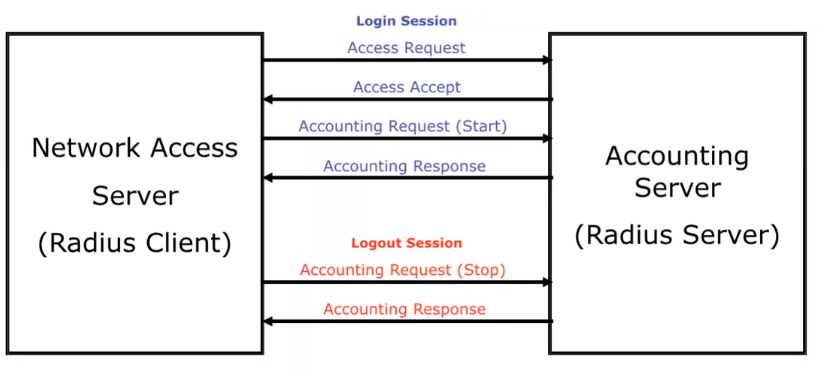
\includegraphics[scale=0.5]{radius.png}
\end{center}
Il \textbf{client} è nella \textbf{centrale dell'operatore}. Client comunica con il server che mantiene info sugli utenti e risponderà si/no per accettare l'autenticazione.\\
Dopo accesso c'è l'accounting request start: da ora navighi e calcolo informazioni per fare "il conto". A fine si manda richiesta di stop e in base a quello si calcola  costo. Quindi c'è comunicazione costante col server RADIUS, in modo da poter interrompere comunicazione se superate eventuali soglie (e non scoprire il superamento solo al logout).\\
Si può solamente fare billing su tempo e durata.
\paragraph{Pacchetti} \begin{center}
	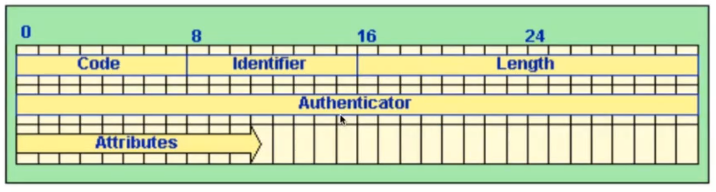
\includegraphics[scale=0.75]{radiuspkt.png}
\end{center}
\begin{list}{}{}
	\item \textbf{Code}: byte contenente il comando/risposta RADIUS
	\item \textbf{Identifier}: byte che identifica il comando/risposta RADIUS
	\item \textbf{Length}: lunghezza del pacchetto
	\item \textbf{Authenticator}: balore usato per autenticare la risposta del server RADIUS
	\item \textbf{Attributer}: attributi del comando/risposta
\end{list}
\chapter{Data Structures}
\paragraph{Bitmap} Array di bit. Lunghezza arbitraria e aggiunta/rimozione in O(1) con operazioni su bit semplici. Memoria in base ai bit usati
\begin{center}
	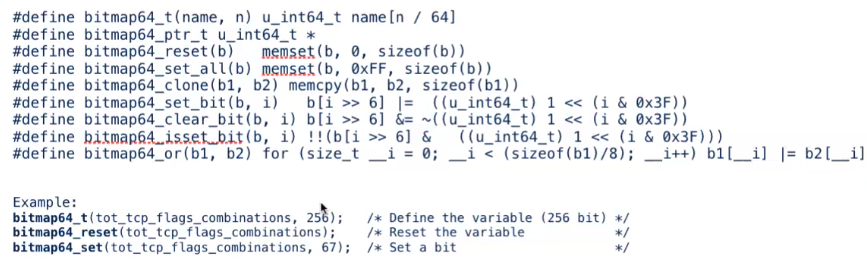
\includegraphics[scale=0.75]{bitmap.png}
\end{center}
\paragraph{Compressed Bitmaps} Una bitmap è un array di bit solitamente di lunghezza predefinita. Utile per specifici domini, possono essere sparse. Es. [0,12,23,500,510,522,10000] maggiorparte a 0 e solo 7 bit a 1. \textbf{Inefficiente}.\\
Si possono comprimere contando il numero di ripetizioni es. 1(1), 11(0), 1(1), 10(0), 1(1), 476(0)\ldots che significa 1 bit a 1, 11 bit a 0\ldots\\
Molte librerie come WAH, EWAH, COMPAX\ldots la maggiorparte non permettono di settare un bit arbitrario "indietro", ma solo in avanti. Se si settano bit solo in avanti si può costruire la bitmap a runtime con memoria minima.\\
Vantaggio: una volta compressa si possono fare AND, OR, NOT senza fare unroll (cioè decomprimere). Una delle più popolari è \texttt{roaringbitmap.org}
\subparagraph{Compressed Bitmap Indexes} 
\begin{center}
	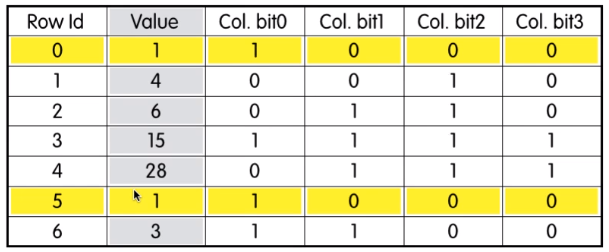
\includegraphics[scale=0.7]{comprbitmapindex.png}
\end{center}
Sono utili per memorizzare dati flussi perché molto efficienti. Nell'esempio si ragiona per colonne, prendo uno dei valori e setto nelle colonne il valore corrispondente nei bit. Creo l'indice bit a bit, e ogni colonna rappresenta il bit $i$-esimo. $n$ colonne, una per bit, se vedo ogni colonna indipendente la posso vedere come una bitmap compressa.\\
Dammi tutte le righe che hanno valore 1: $C_0 = 1$ AND $C_1 = 0$ AND $C_2 = 0$ AND $C_3 = 0$\\
Estremamente veloci, molto più delle bitree su dimensioni notevoli. Altra proprietà: per trovare indirizzi nelle netmask (tutte colonne che fanno parte della maschera settati come voglio), oppure mettere in AND due righe per prendere quelle che si intersecano su valori che voglio.
\paragraph{Bloom Filters} I bloom filters sono strutture dati probabilistiche che rispondono alla domanda: elemento appartiene a set? Risponde con una certa probabilità.\\
Si può rispondere a questa domanda con altre strutture dati, come hash o bitmap molto lunghe, al prezzo di un costo molto maggiore perché in quei casi si analizzano dati raw.\\
Sono array di bit di lunghezza $m$, settando i bit usando almeno due funzioni hash indipendenti e uniformemente distribuite $h_1()$ e $h_2()$. Se voglio aggiungere $\alpha$, faccio $h_1(\alpha)$ e setto i bit che vengono fuori, poi $h_2(\alpha)$ e setto i bit. Per vedere se $\beta$ è presente, faccio le due hash e vedo se i due bit sono stati settati, allora \textbf{certa probabilità} che $\beta$ appartiene, se uno o nessuno dei due \textbf{non} è settato allora sicuramente non appartiene.\\\\
La probabilità non è uno svantaggio, perché permette di fare ricerche molto veloci. Essendo probabilistica \textbf{non posso avere la certezza}.
\begin{center}
	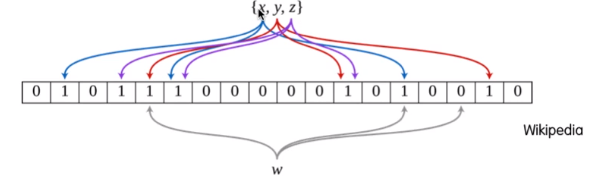
\includegraphics[scale=0.85]{bloomfilters.png}
\end{center}
Con i \textbf{counting bloom filters} rimpiazzo il vettore di bit con un intero per sapere quanti bit sono settati o quante volte è stato settato un bit. Più memoria, ma si possono rimuovere elementi (con i bloom non si può).\\
Buoni hash sono murmur, nfv e md5.
\paragraph{Trie} Pronunciato try, (pun su \textit{re\underline{trie}val} e \textit{tree}). Albero non basato su comparazioni, ogni nodo ha etichetta.
\begin{center}
	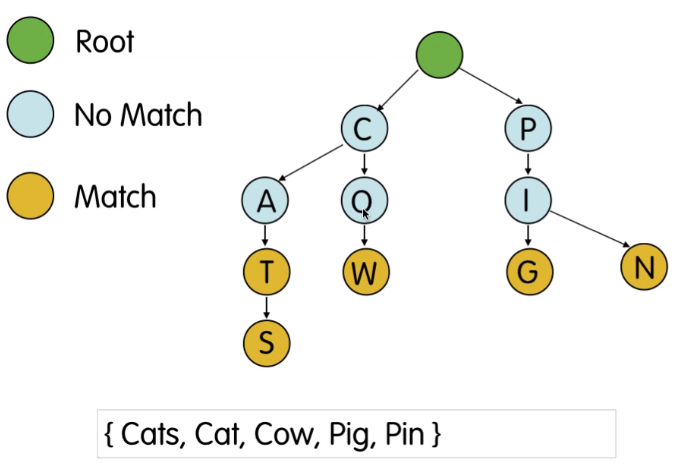
\includegraphics[scale=0.5]{tries.png}
\end{center}
Nodi aggiunti/rimossi/cercati. Possibilità di cercare stringhe che iniziano per prefissi, e generare stringa in ordine di dizionario (se link in ordine alfabetico)
Performance in $O(w)$ dove $w$ è lunghezza dell'albero.
\subparagraph{Radix tree} Come trie ma nodi collassati
\begin{center}
	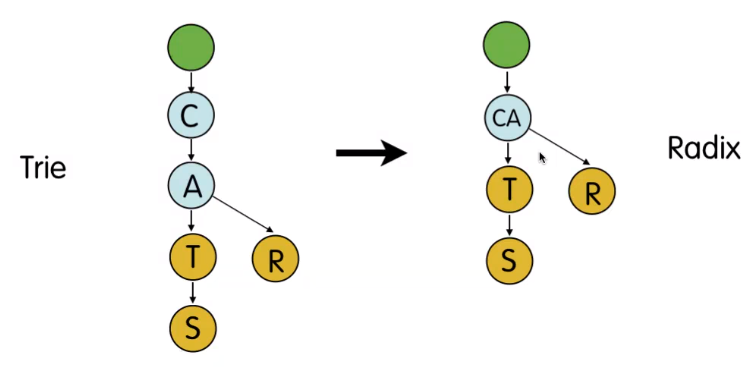
\includegraphics[scale=0.5]{radixtrie.png}
\end{center}
\subparagraph{Patricia Tree} Numeri invece di stringhe, ogni nodo contiene una parte di indirizzi IP.\\
Struttura dati di riferimento per subnetting match su IPv4/IPv6.\\
codice su \texttt{github.com/ntop/nDPI/blob/dev/src/lib/third\_party/src/ndpi\_patricia.c}
\paragraph{Entropia} Entropia misura usata per misurare come i dati sono distribuiti su un certo range. Più alta entropia più dati sono sparpagliati.\\
Formula \texttt{csrc.nist.gov/csrc/media/publications\ldots}\\
Esempio per usarla: grado di quanto sono distribuiti i dati\\
Esempio di uso sul TLS: entropia dei byte prima e dopo crittografia cambia ma è sempre compresa fra delle soglie per dati omogenei. Tramite entropia si può capire il tipo di dato.
\chapter{Network Traffic Monitoring su Container}
Traffic monitoring: garantire disponibilità fiunzionamento a lungo termine. A inizio 2000 fondamentalmente solo SNMP. Misure volumetriche, con RMON poco di più: sempre aggregate. Successivamente sFlow (2001) per risolvere problema visibilità: sempre contatori ma con informazioni di contesto.\\
Si dice che \textit{i pacchetti non mentono mai}, info utili per capire: problemi di traffico, traffico non conforme a politiche\ldots\\
Sempre pacchetti e flussi. Non sono sbagliati i pacchetti, ma il problema è che bisogna adattarsi ai pacchetti. Paradigma utile per monitorare in maniera passiva, ma la crittografia ad esempio crea problemi. Non è \textbf{naturale per le persone}.
\paragraph{System Introspection} Senza catturare traffico di rete chiedo al sistema. Ma ho comunque bisogno di info di contesto.\\
Adesso monitoraggio \textbf{unificato}: sempre parte classica (NetFlow, SNMP, IPFIX) ma con anche strumenti moderni per ambienti in container.
\section{eBPF}
macchina virtuale semplice eseguita nel kernel linux\\
codice eseguito nel kernel space
\paragraph{Kprobe} Kernel Probe. Permette di collegare ad un qualsiasi indirizzo di memoria d'istruzione del kernel un custom hook, cioè codice utente eseguito quando viene eseguita quell'istruzione, con visibilità completa di quella funzione kernel.
\begin{center}
	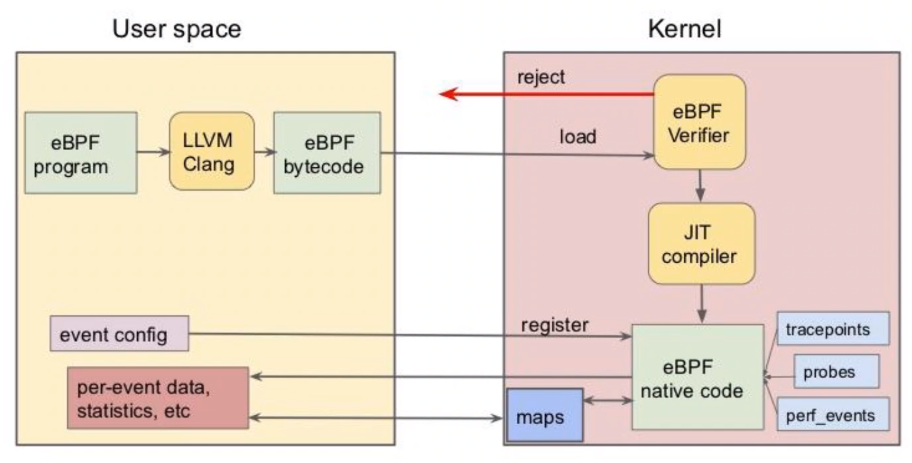
\includegraphics[scale=0.75]{ebf.png}
\end{center}
eBPF verifier: rigetta tutto ciò che non reputa adatto ad essere eseguito in kernel space. serie di condizioni per verificare che sia adatto: no loop indefiniti, ricorsione limitata, limitazione in spazio, no variabili globali, no allocazione dinamica, numero massimo istruzioni.
\paragraph{Container} Istanze utente isolate, ognuna possibilmente su un processo diverso. Solitamente sfruttano feature del kernel: cgroup (limiti a risorse usabili per singoli processi), namespace (gruppi a cui iscriversi per avere vista limitata del sistema)
\end{document}